\documentclass[specification,annotation,times]{itmo-student-thesis}

\usepackage{subcaption}

\newcommand{\revise}[1]{{\color{red!70!black} #1 }}

%% Опции пакета:
%% - specification - если есть, генерируется задание, иначе не генерируется
%% - annotation - если есть, генерируется аннотация, иначе не генерируется
%% - times - делает все шрифтом Times New Roman, требует пакета pscyr.

%% Указываем файл с библиографией.
\addbibresource{wjf-thesis.bib}

\begin{document}

\studygroup{M4236}
\title{Разработка эффективной структуры данных, поддерживающей инкрементальные изменения, для параллельной обработки деревьев}
\author{У Цзюньфэн}{У Цзюньфэн}
\supervisor{Станкевич Андрей Сергеевич}{Станкевич А.С.}{канд. техн. наук, без звания}{доцент кафедры компьютерных технологий Университета ИТМО}
\publishyear{2016}

\addconsultant{Буздалов М.В.}{канд. техн. наук, без звания}

%% Задание
%%% Техническое задание и исходные данные к работе
\technicalspec{Требуется разработать структуру данных для параллельной обработки деревьев, поддерживающую инкрементальные изменения (добавление нового узла, подвешивание узла в качестве ребенка другого 
узла, отцепление узла от его родителя, изменение меток на вершинах и ребрах). В разработанной структуре данных требуется снять ограничение на максимальную 
степень вершины, имеющееся у существующих реализаций. Требуется поддержка эффективного выполнения запросов на определения корня дерева по представителю дерева,
определение групповой суммы меток в поддереве данной вершины и на пути между двумя данными вершинами. При этом требуется поддерживать произвольные типы меток на вершинах и ребрах, являющихся 
моноидами (произвольный моноид для ребер и коммутативный для вершин). Структуру данных требуется реализовать на языке C++ с использованием библиотеки PASL для реализации параллельных операций.}

%%% Содержание выпускной квалификационной работы (перечень подлежащих разработке вопросов)
\plannedcontents{\begin{enumerate}
    \item обзор источников с целью выявления наиболее перспективной структуры данных для поддержки операций с динамическими деревьями;
    \item реализация выбранной структуры данных в виде контейнера языка C++, поддерживающего необходимые запросы, а также применяемые пакетами операции модификации;
    \item реализация эффективного параллельного применения пакетов операций модификации;
    \item экспериментальные исследования эффективности разработанной реализации.
\end{enumerate}}

%%% Исходные материалы и пособия 
\plannedsources{\begin{refsection}
\nocite{sleator83,reif94,acar04}
\printannobibliography
\end{refsection}}
%%% Календарный план
\addstage{}{}

%%% Цель исследования
\researchaim{Разработка структуры данных на основе Rake-and-Compress деревьев для параллельной обработки деревьев, поддерживающей инкрементальные изменения: добавление нового узла, подвешивание узла в 
качестве ребенка другого узла, отцепление узла от его родителя, изменение меток на вершинах и ребрах.}

%%% Задачи, решаемые в ВКР
\researchtargets{\begin{enumerate}
    \item снятие ограничения на число детей вершины, присущее параллельным реализациям Rake-and-Compress деревьев;
    \item уменьшение использования памяти с $\Theta(n \log n)$ до $\Theta(n)$, где $n$~--- общее число вершин в деревьях, при сохранении эффективности параллельных операций;
    \item обеспечение поддержки меток произвольных типов для вершин и ребер, при условии что метки на вершинах являются элементами коммутативного моноида, а метки на ребрах~---
          элементами произвольного моноида.
\end{enumerate}}

%%% Использование современных пакетов компьютерных программ и технологий
\advancedtechnologyusage{В реализации был использован язык C++ стандарта C++11. Для обеспечения целостности и надежного хранения кода использовалась система контроля версий Git.
Для реализации параллельных операций использовалась библиотека Parallel Algorithm Scheduling Library (PASL).}

%%% Краткая характеристика полученных результатов 
\researchsummary{Разработана эффективная реализация Rake-and-Compress деревьев. Ограничение на число детей вершины снято путем раздваивания каждой вершины и
организации декартова дерева для детей каждой вершины. Использование памяти уменьшено до $\Theta(n)$ при сохранении эффективности параллельных операций
путем хранения вершин в контейнерах переменной длины (векторах) отдельно для четных и нечетных раундов сжатия Rake-and-Compress деревьев, что позволило разделить
области памяти для чтения и для записи различными потоками.}

%%% Гранты, полученные при выполнении работы 
\researchfunding{гранты отсутствуют.}

%%% Наличие публикаций и выступлений на конференциях по теме выпускной работы
\researchpublications{
\begin{refsection}
По теме выпускной работы были сделаны выступления на двух всероссийских конференциях, по итогам которых
имеются следующие публикации:\nocite{wjf-kmu, wjf-spisok}
\printannobibliography
\end{refsection}
}

%% Эта команда генерирует титульный лист и аннотацию.
\maketitle{Магистр}

%% Оглавление
\tableofcontents

%% Макрос для введения. Совместим со старым стилевиком.
\startprefacepage

Структуры данных для поддержания динамических деревьев имеют прямое приложение к эффективному решению многих практическим задач,
таких как поиск максимального потока~\cite{goldberg88}. Такие структуры данных должны поддерживать лес деревьев на заданных вершинах,
операции обновления (добавление и удаление ребер, а в случае укорененных деревьев~--- подвешивание вершины к вершине и отцепление вершины).
Также, как правило, на вершинах, ребрах, или и тех, и других имеются пометки. Структуры данных также должны уметь отвечать на запросы
вида <<достижима ли вершина $A$ из вершины $B$ по ребрам деревьев>>, <<найти длину пути из вершины $A$ в вершину $B$>>,
<<найти сумму пометок на пути из вершины $A$ в вершину $B$>>, <<найти сумму пометок в поддереве вершины $A$>> и другие.
С практической точки зрения, полезно также уметь строить такие структуры данных параллельно,
а также параллельно применять совокупности, или пакеты, операций обновления.

Впервые задача поддержания динамических деревьев была поставлена в работе Слейтора и Тарьяна~\cite{sleator83}, в которой была предложена
структура данных, известная сейчас как ST-дерево или Link-Cut дерево. Эта структура данных поддерживает операции добавления и удаления ребер.
Также она поддерживает пометки на ребрах и запросы вида <<найти сумму пометок на пути из одной вершины в другую>>.

В то же время в ряде работ~\cite{miller85, miller89, miller91, reif94} Миллером и Рейфом был разработан подход параллельной обработки деревьев,
известный как <<параллельное сжатие деревьев>> (англ.~Parallel Tree Contraction). Суть этого подхода заключается в построении структуры данных,
описывающей данное дерево и позволяющей выполнять запросы различного вида на этом дереве, таким образом, чтобы основная часть работы выполнялась
параллельно. Тем самым, при наличии многопроцессорных вычислительных систем, сокращается время между получением входных данных и моментом, начиная
с которого возможно эффективное выполнение запросов к дереву.

Различные варианты параллельного сжатия деревьев применяются для реализации динамических деревьев для ускорения применения изменений при наличии
многопроцессорных вычислительных систем. Так, известны структуры данных Topology Trees~\cite{frederickson97}, Top Trees~\cite{alstrup05} и RC-Trees~\cite{acar03},
поддерживающие параллельное построение, при этом 
некоторые из них также поддерживают применение различных операций модификации, в том числе параллельно. 
В работе~\cite{acar04} исследовалась возможность добавления поддержки инкрементальных изменений дерева путем привнесения идей
из работы~\cite{miller85}. В то же время, эти структуры накладывают различные ограничения на вид поддерживаемого дерева или на поддерживаемые операции модификации.

\paragraph{Мотивация.}

Задача поддержки динамических деревьев все еще не может считаться решенной удовлетворительно. Так, многие из существующих структур данных не поддерживают параллельное
обновление, работу с метками на ребрах или на вершинах, агрегационные запросы на путях или поддеревьях, или работу с деревьями, имеющими вершины произвольной степени.
Остается открытым также вопрос эффективной реализации таких структур данных~--- в частности, по времени выполнения запросов, времени применения операций обновления,
используемой памяти, использованию кешей различных уровней, эффективности использования ядер многопроцессорных систем.

Кроме того, для структур данных, поддерживающих параллельное построение или обновление, отсутствуют их реализации, удобные для использования в приложениях.
Существующие программные реализации имеют исключительно исследовательский характер и трудны для переиспользования, в то время как для пользователей
была бы удобна реализация, устроенная по образцу контейнеров или коллекций из стандартных библиотек языков программирования (таких как
\texttt{std::vector} в \emph{C++} или \texttt{java.util.ArrayList} в \emph{Java}).

Контейнерную реализацию дополнительно усложняет тот факт, что использование отложенного обновления (в том числе параллельного) требует от структуры данных
поддержки в том или ином виде минимум двух версий данных~--- последней стабильной версии и текущей версии, содержащей еще не примененные изменения.
В дополнение к этому, вновь применяемые изменения крайне желательно проверять на корректность, причем в некоторых случаях такая проверка может занимать большую часть
времени работы со структурой данных, поэтому также требуется предусмотреть режим, в котором корректность не проверяется.

Наличие указанных проблем мотивируют создание эффективной реализации структуры данных, поддерживающей параллельное применение пакетов изменений,
реализованной в виде переиспользуемого обобщенного контейнера данных, поддерживающего опциональную проверку корректности применяемых изменений.

\paragraph{Цели исследования.}

\revise{
В этой диссертации, преимущества RC-Trees и анализируются требованию к разработке новой структуры данных на 
основе структуры данных RC-Trees для решения динамических задач оцениваются.

Общая цель диссертации заключается в разработке и реализации эффективного параллельного алгоритма для 
контракции дерева поддержки инкрементных изменений данных. 

Специально, во-первых, улучшить базовую структуру данных RC-Tree для поддержки коммутативных и некоммутативных 
данных, а также направленной и ненаправленной функций. 

Во-вторых, реализовать алгоритм, который должен эффективно работает. 

В-третьих, разработать алгоритм в параллельном процессе, и оценить эффективность. Для решения динамических 
задач в параллельных вычислениях нужна параллельная библиотека, в этой диссертации, известная параллельная 
была библиотека Openmp и параллельная библиотека называется PASL, которая обозначает Parallel Algorithm 
Scheduling Library, используется для оценки эффективности параллельных вычислений. 

Основной проблемой исследования является то, что какая структура данных может быть использована для достижения 
целей и какие ограничения существуют?

Второй проблемой исследования является то, что какой алгоритм, основанный на структуре данных решает вопросы 
на динамическом задаче дерева?
}

\paragraph{Ожидаемые результаты.}

\revise{
Применения параллельного контракции дерева описаны в диссертации могут  использовать для оцеки эффективности 
структуры данных. Одна проблема, что параллельная контракция дерева может решить это было change propagation~\cite{acar05}.
Change propagation автоматически регулирует выход алгоритма к изменению входного. Другая 
проблема, которая решает контракцию дерева это вычисление выражения, выполняя контракция дерева в параллель 
сделало бы вычисления более эффективно.

Ожидаемым результатом этого диссертации являются решения проблемы исследования и достижения цели. Точные 
ожидаемые результаты следует, сначала новая структура данных разработан на основе RC-Tree, и он поддерживает 
требуемый тип данных. Эффективность новой структуры данных должна быть приемлемыми в последовательном 
вычислений. Во-вторых, там будет включение, чтобы выбрать время вычислений со структурой данных для ответа на 
запросы, варианты должны быть последовательными, параллельно с Openmp и параллельно с PASL. В-третьих, оценка 
эффективности с различным вычислительным типом должна быть приемлемыми. Алгоритм работает в параллельном 
процессе должен отвечать на запросы быстрее, чем алгоритм без параллельно. Потому что если затраты времени 
несоответствие двух не очень много, реализация не имеет смысла.

В общем и целом, ожидаемым результатом является улучшение базовой структуры данных, реализация развитого 
структуры данных, эффективность структуры данных удовлетворяющих и вопросы исследования отвечают в 
диссертации.
}

%% Начало содержательной части.
\chapter{Обзор источников}

В данной главе приведен обзор литературных источников, используемых в настоящей работе. 
В разделе~\ref{survey-tree} описывается задача поддержания динамических деревьев и известные структуры данных для решения этой задачи.
В разделе~\ref{survey-contraction} описываются алгоритмы параллельного сжатия деревьев.
В разделе~\ref{survey-misc} описываются вспомогательные алгоритмы и структуры данных, которые будут использованы при решении задач, поставленных в настоящей диссертации.

\section{Методы решения задачи поддержания динамических деревьев}\label{survey-tree}

Структуры данных для поддержания динамических деревьев имеют прямое приложение к эффективному решению многих практическим задач,
таких как поиск максимального потока~\cite{goldberg88}. Такие структуры данных должны поддерживать лес деревьев,
операции обновления (добавление и удаление ребер, а в случае укорененных деревьев~--- подвешивание вершины к вершине и отцепление вершины).
Также, как правило, на вершинах, ребрах, или и тех, и других имеются пометки. Структуры данных также должны уметь отвечать на запросы
вида <<достижима ли вершина $A$ из вершины $B$ по ребрам деревьев>>, <<найти длину пути из вершины $A$ в вершину $B$>>,
<<найти сумму пометок на пути из вершины $A$ в вершину $B$>>, <<найти сумму пометок в поддереве вершины $A$>> и другие.
С практической точки зрения, полезно также уметь строить такие структуры данных параллельно, а также параллельно применять совокупности, или пакеты, операций обновления.

\subsection{Link-Cut Trees}

\revise{
ST-Tree является лучшим известная структура данных для решения динамических задач, представлен по Sleator D D, Tarjan R E. (1983). В идее этой структуры данных, ссылка и вырезание операции имеют важное 
значение, В результате структура данных также известен как link-cut trees.
}

\revise{
ST-Trees совершают операции на корневом дереве, корень дерева имеют только дети и без родителей. Три операции вводятся в структуре данных: link (v, w) операция, что делает связь между корневой v дерева и 
вершины w из другого дерева, добавив ребро (v, w), и делает w быть родителем v; cut(v) операция удаляет ребро между вершиной v и его родителем, затем делит дерево на два дерева. В частности, вершина v не 
может быть корнем дерева; evert (v) операция делает вершина быть корнем, чтобы превратиться в новое дерево, а корень будет вершина в новом токарной дереве. Операции с Link-Cut деревом изображены на 
рисунке~\ref{fig:link-cut-tree}.
}

\begin{figure}[!ht]
\centering
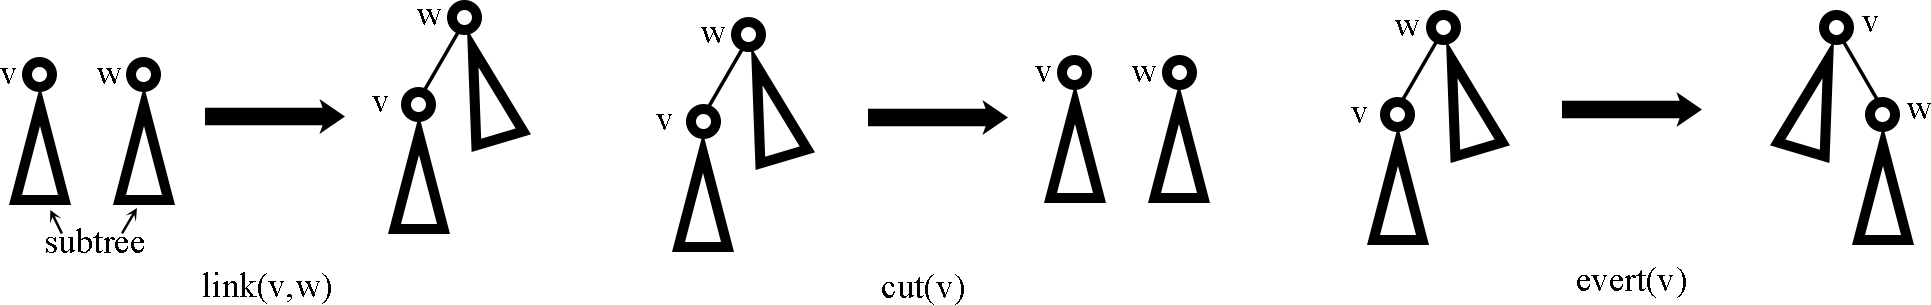
\includegraphics[width=\textwidth]{pic/link-cut-tree.png}
\caption{Операции Link-Cut деревьев: \texttt{Link}($v$, $w$), \texttt{Cut}($v$), \texttt{Evert}($v$)}\label{fig:link-cut-tree}
\end{figure}

\revise{
ST-Trees поддерживают операций пути, время затраты O (log n) времени за одну операцию на вес сбалансированного дерева в худшем случае, и O (log n) время на одну операцию на скошенного дерева в 
амортизационной времени случае. ST-Trees может также поддерживать другие запросы, но информация должна быть только агрегируются над путями. 
ST-Trees были первыми, чтобы сделать время срабатывания для динамического дерева в логарифмическое время, которые дают основную концепцию развития структуры данных для решения динамических задач.
}

\subsection{Topology Trees}

\revise{
Первая структура данных контракция на основе является Topology Trees, который ввел по Frederickson, G. N. (1997). Topology Tree является поддержкое дерево.
С учетом поддержки дерев S базового дерева T. Каждый узел в S является поддеревом в T, и кластер из S является поддерево, соответствующий узлу в S. Дерево Т' представляет собой кластер из S. Ребро в Т 
прилегающий ребро Т'. Степень Т' является число прилегающего ребра. Вершина кластера Т' из S является граничной вершиной, если она имеет прилегающий ребро. Число граничных вершин кластера Т' является 
размер граница его. (Acar U.et al. 2003).
}

\begin{figure}[!ht]
\centering
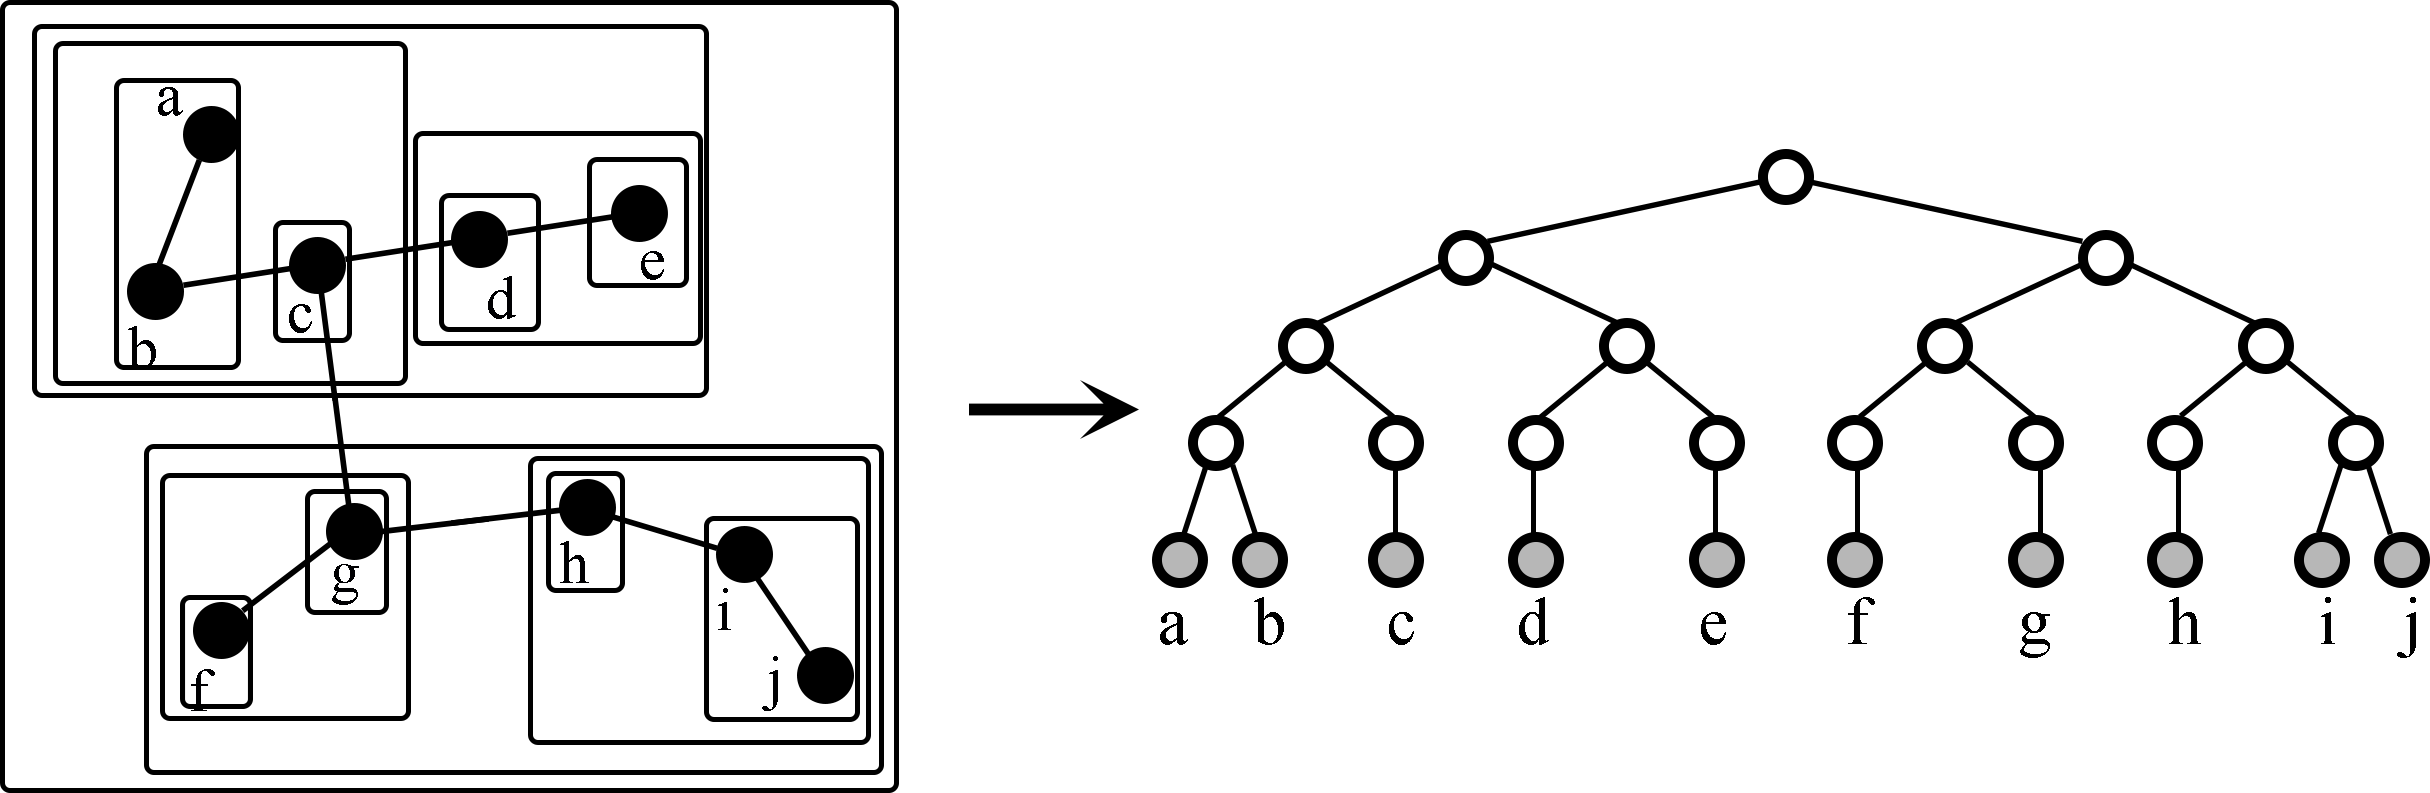
\includegraphics[width=\textwidth]{pic/topology-tree.png}
\caption{Пример Topology Tree}\label{fig:topology-tree}
\end{figure}

\revise{
Frederickson, G. N. (1997) ввел Topology Trees интерпретировать кластер как вершины вместо ребер в качестве опорного дерева. В Topology Trees, кластер имеет не более чем на три градуса. Направленная 
Topology Trees структура данных разработана для поддержания динамически бинарных деревьев. Время работы это занимает O (log n), где n является количество вершин в деревьях. Topology Trees являются 
внедрение link cut trees, так что основные операции в Topology Trees также ссылку и вырезанию операции. 
Хотя Topology Trees делают контракцию динамического дерева проще, с учетом алгоритма, его требование для всех вершин в лесу, чтобы иметь степень ограничена константой, ограничивает развитие само по себе. 
Для осуществления работы алгоритма более эффективно, структура данных должна поддерживать изменяемую степень вершин в дереве поддержки.
}

\subsection{Top Trees}

\revise{
Структура данных Top Trees представляет собой структуру данных разработан на основе двоичного дерева для некорневых динамического деревьев (Alstrup S. et al. 1997). В некорневого дереве, ребра, смежные с 
каждой вершины произвольно расположены в фиксированном круговом порядке. Кластера в Top Trees является поддеревом пути первоначального базового дерева. В Top Trees кластеры имеют граничный размер не более 
двух. Когда операция контракция вычисляется, он занимает O (log n) время, и преимущество состоит в том, что время стоимость O (log n) с произвольной степенью дерева. Ограничение Top Trees является то, что 
он поддерживает только бинарное дерево.
}

\revise{
Контракция дерева выполняет операции, чтобы сделать все кластеры в опорном дереве в единый кластер. Top Trees поддерживет контракцию для бинарного дерева. Два кластера (u, v) и (v, w) могут быть 
объединены, если v является общим концом этих двух кластеров и имеет степень двух. Alstrup S. et al. (1997) использует концепцию компресса, объединенный кластер (u, w) из двух кластеров называется 
компресс кластера. Затем, если (w, x) является преемником (v, x) и v имеет степень один, эти кластеры могут быть объединены в кластер Рейк. После комбинации, Рейк кластер имеет конечные точки w и x. 
Каждый рейк или компресс кластер может рассматриваться как родитель, который агрегирует информацию, содержащуюся в ее детей. Корень верхнего дерева представляет собой кластер, который весь лежащий в 
основе дерева. Для динамического изменений по сравнению с лежащей в основе дерева, например, link или cut операции производятся, структура данных просто обновляет контракцию пострадавших. 
}

\revise{
В качестве приложения структуры данных, он отвечает на запросы динамической задачи. Когда запрос пути выполняется, например, она задает путь между вершиной V и W, expose (v, w) операция быть использовано, 
которая возвращает корневой кластер с V и W в качестве конечных точек, и если v и w не в том же дереве, операция будет возвращать нуль. Однако, даже если v и w находятся в том же дереве, контракция в 
верхнем дереве может потребоваться изменить, потому что корень кластера станет путь от v до w. Top Trees поддерживает агрегацию по путям или деревьев напрямую. Они не требуют степень вершины, что делает 
преимущество, чем Topology Trees. 
}

\subsection{RC-Trees}

Структура данных Rake-and-Compress Tree~\cite{reif94}~--- одна из наиболее подходящих структур данных для решения задач настоящей диссертации,
теоретически поддерживающая параллельное построение и параллельное обновление (включая не только добавление и удаление листьев дерева, но и произвольные
подвешивания и отцепления вершин), а также запросы как на путях, так и на поддеревьях.

Идея Rake-and-Compress деревьев, в изложении для укорененных деревьев, заключается в следующем. Для дерева последовательно строится несколько <<уменьшенных>> копий дерева, причем $i$-тая копия получается
из $(i-1)$-ой применением ко всем допустимым вершинам одной из следующих операций:
\begin{itemize}
    \item Rake. Вершина, имеющая родителя и не имеющая детей, удаляются вместе с ребром, ведущим к родителю (рисунок~\ref{fig:rake}).
    \item Compress. Вершина, имеющая родителя и ровно одного ребенка, удаляется вместе со смежными ребрами, а вместо этого ребро проводится от ребенка удаляемой вершины к родителю этой вершины
          (рисунок~\ref{fig:compress}). При этом родитель не должен подвергаться операции Compress, а ребенок не должен подвергаться ни операции Compress, ни операции Rake.
\end{itemize}

\begin{figure}[!ht]
\centering
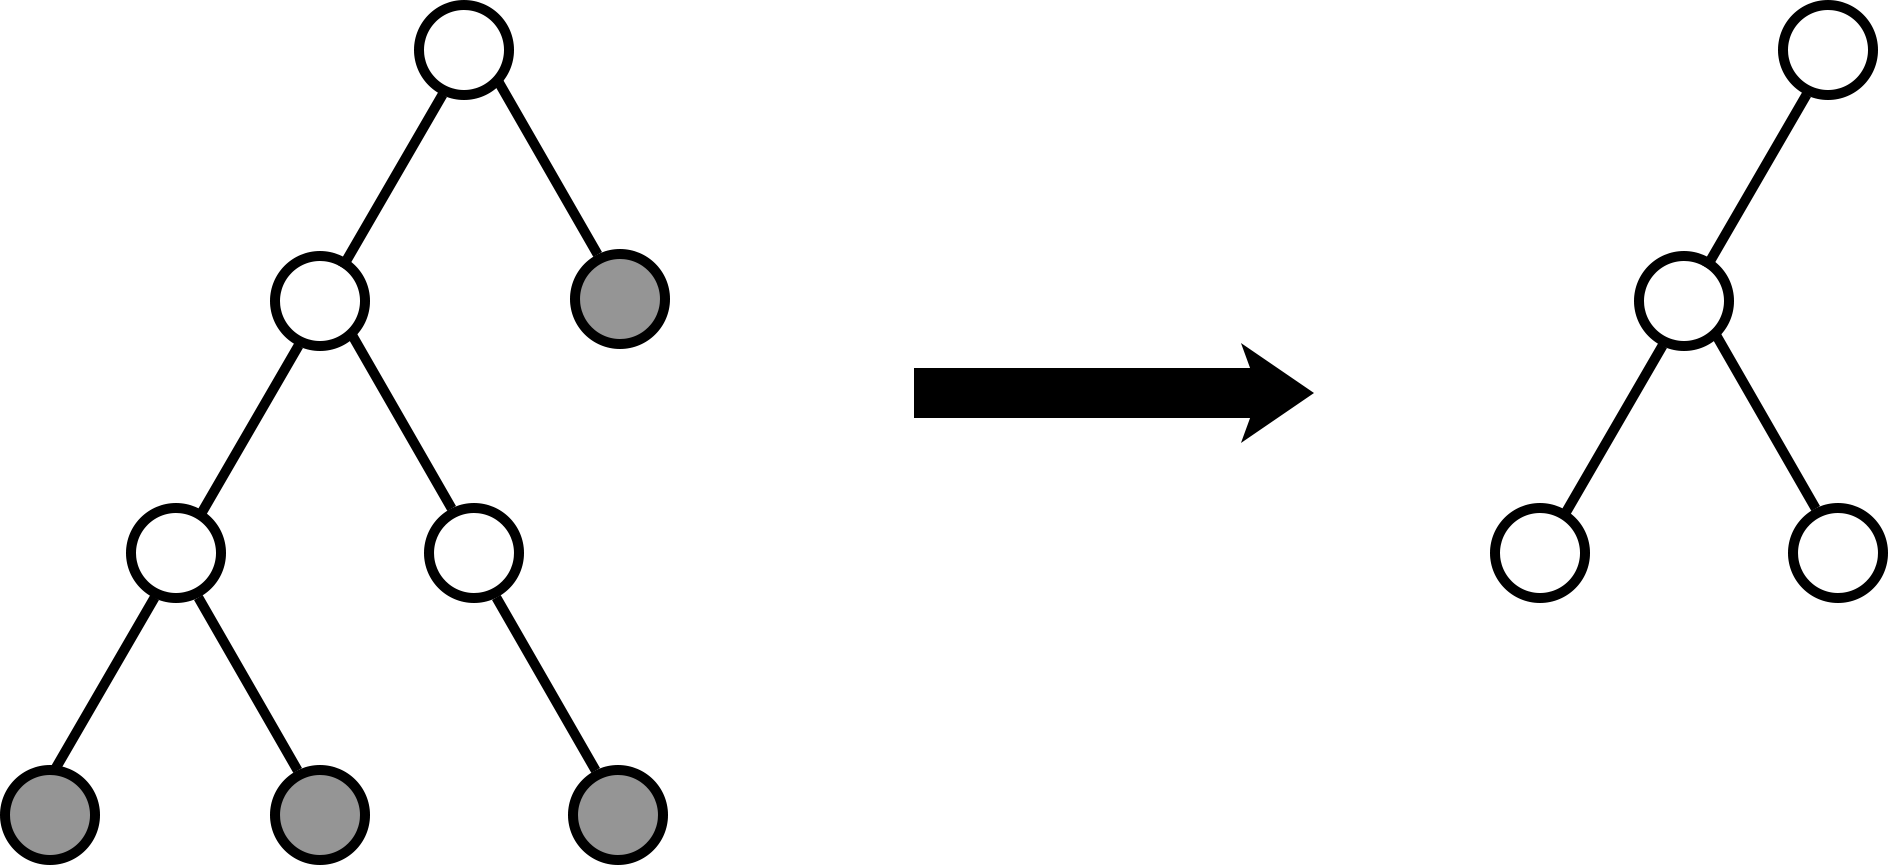
\includegraphics[width=0.5\textwidth]{pic/rake.png}
\caption{Операция Rake}\label{fig:rake}
\end{figure}
\begin{figure}[!ht]
\centering
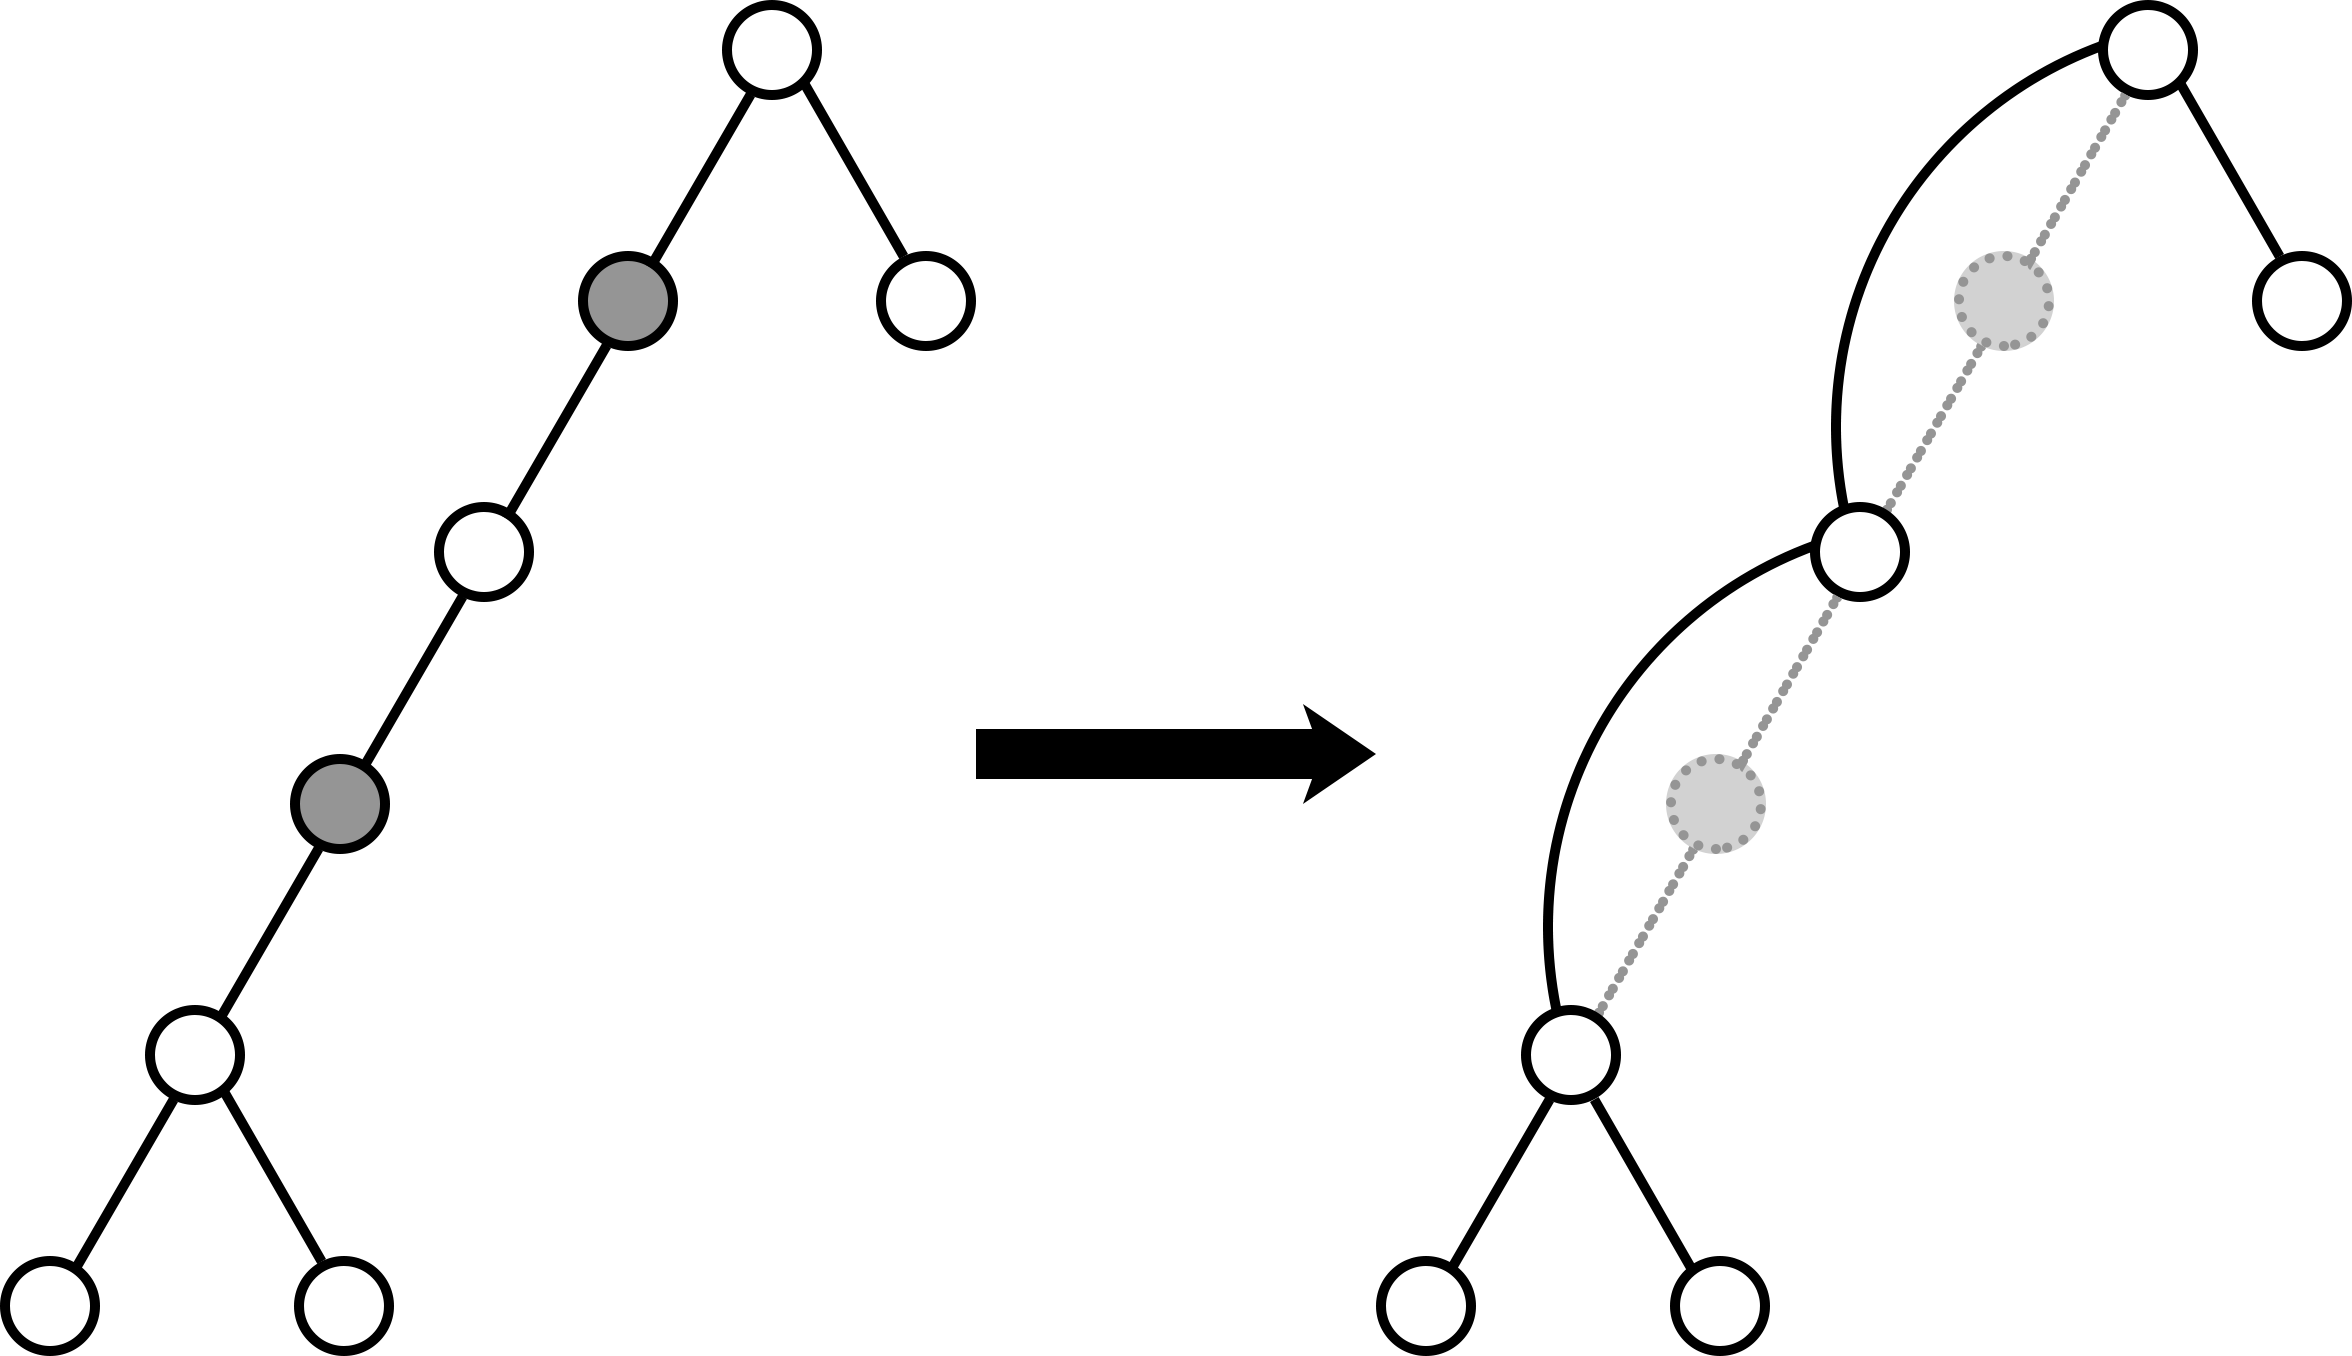
\includegraphics[width=0.5\textwidth]{pic/compress.png}
\caption{Операция Compress}\label{fig:compress}
\end{figure}

С каждым раундом число вершин в дереве, если оно больше единицы, уменьшается как минимум в $8/7$ раз в каждой компоненте связности. В конце работы для каждой компоненты связности
остается ровно одна вершина, для чего требуется произвести $O(\log n)$ раундов (рисунок~\ref{fig:rctree-overall}). RC-дерево можно представить как дерево с двумя типами вершин~--- первый тип соответствует 
вершинам оригинального дерева, второй тип~--- его ребрам (рисунок~\ref{fig:rctree-two-types}).

\begin{figure}[!ht]
\centering
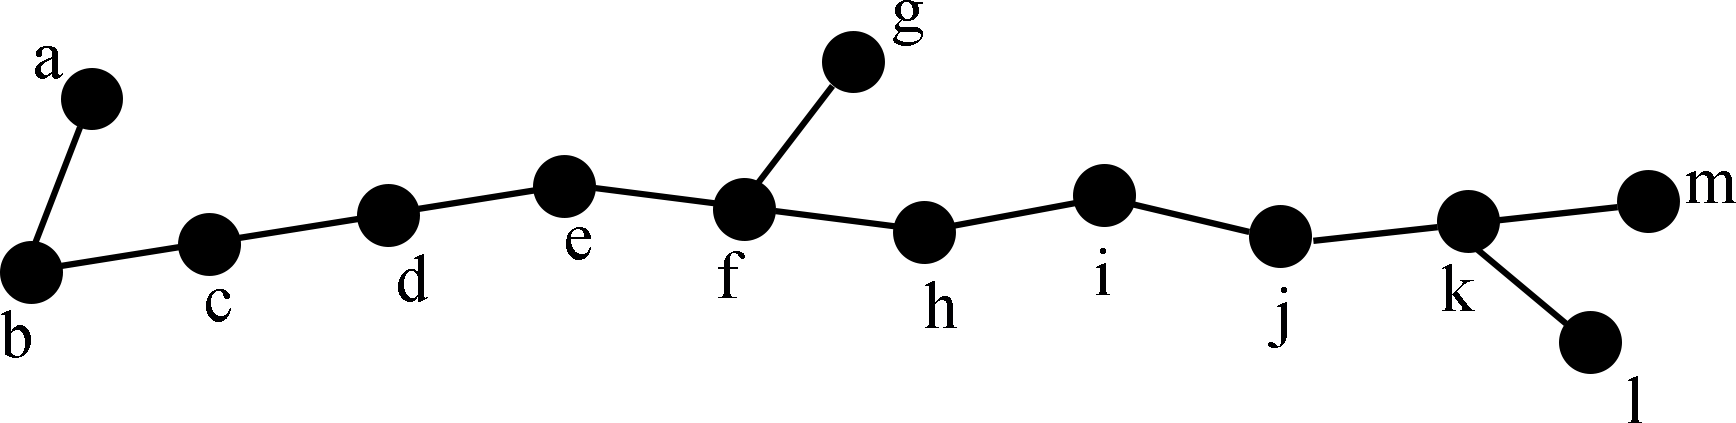
\includegraphics[width=0.5\textwidth]{pic/rc_tree_1_primitive_tree.png}\\

\includegraphics[width=0.75\textwidth]{pic/rc_tree_2_completed_clustering.png}
\caption{Исходное дерево и группировка вершин, полученная последовательным применением операций Rake и Compress}\label{fig:rctree-overall}
\end{figure}

\begin{figure}[!ht]
\centering
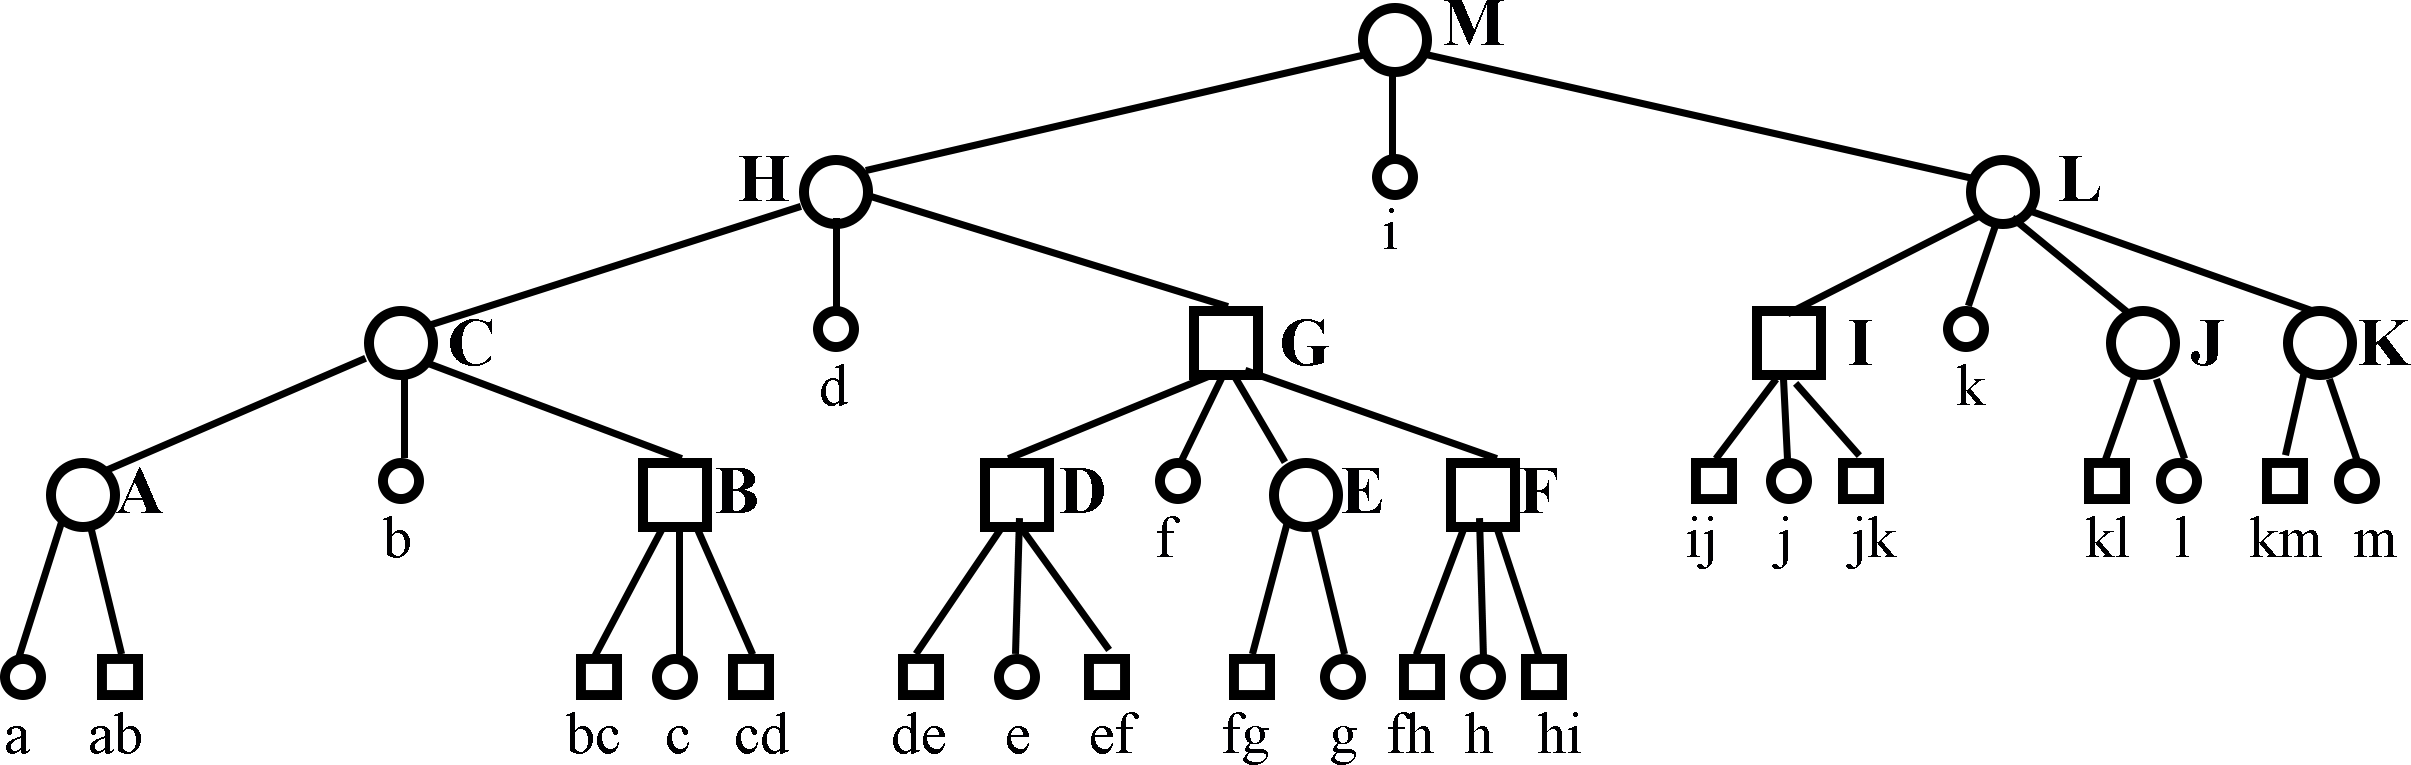
\includegraphics[width=\textwidth]{pic/rc_tree_4_two_types.png}
\caption{Представление RC-дерева как дерева с двумя типами вершин, соответствующим вершинам (круглые вершины) и ребрам (квадратные вершины) оригинального дерева}\label{fig:rctree-two-types}
\end{figure}

Такое многоуровневое представление дерева позволяет отвечать на запросы на путях и поддеревьях за время, пропорциональное числу раундов (а следовательно, $O(\log n)$),
даже если дерево изначально было несбалансировано (например, существенно вытянутое). В то же время решение о выполнении операции Rake или Compress можно сделать на основе локальной информации (о самой
вершине и ее ближайших соседях), что позволяет эффективно распараллеливать операции в рамках каждого раунда.
Эффективное применение операций обновления также возможно с использованием этой структуры данных~\cite{acar04}.

\section{Алгоритмы параллельного сжатия деревьев}\label{survey-contraction}

\revise{
Динамические структуры данных дерева решенит задач динамических дерева в последовательных операций. Тем не менее, контракция дерева делает эти структуры данных работают более эффективно, контракция дерева 
является операция для заражения дерева путем удаления некоторых из узлов (Atallah, M. J. (Ed.). 1998). Произведить поддержку контракции дерева изменяемых процессоров~\cite{miller85, miller89},
впервые ввели контракция параллельного дерева и далее обсуждаются в статьях~\cite{miller91, reif94}. Контракция параллельного дерева представляет собой 
структуру, которая поддерживает эффективные параллельные алгоритмы на деревьях~\cite{morihata08}. Эффективный алгоритм параллельно дерева контракция обеспечивает возможность собирать 
значения в дереве эффективно и без конфликта, в результате, приводит к нескольким эффективных параллельных алгоритмов~\cite{morihata11}.
}

\revise{
Контракция параллельного дерева является подход снизу вверх при обработке деревьев. Это делает внедрение новых алгоритмов, облегчающие проще с меньшим количеством процессоры и меньше времени, и делает 
сложные задачи проще с помощью параллельных алгоритмов~\cite{miller85}. Контракция параллельного дерева занимает O (log N) параллельные шаги для базовой структуры дерева, независимо от его 
формы, и это ускоряет операции~\cite{morihata14}.
}

\revise{
При контракции параллельного дерева, существуют две абстрактные операции, выполняемые на деревьях,~\cite{miller85} назвал их Рейк и Компрессия. Рейк операция, которая перемещает все листья с 
дерева T. Компрессия операция, чтобы удалить все максимальные цепи дерева Т в одном шаге, максимальная цепь здесь означает, что каждый узел имеет родителя и одного ребенка, последний узел цепь имеет 
ребенка, и этот ребенок не является листом. Если коротко, то операция компресса удаляет каждые два ребра между двумя узлами в цепи дерева T. Другими словами, например, в бинарном дереве, операция 
компресса удаляет узел, который только есть один ребенок и его родитель имеет его как единственный ребенок. Дополнительная операция, контракция, является одновременное применение Рейк и Компресс операции 
по всему дереву. Задача для сокращения дерева, чтобы уменьшить дерево к одному узлу. Во-первых, следует определить корневое дерево T с n узлами и корнем r. Для выполнения контракции, Рейк операции и 
Компресс операции выполняются в любом порядке и в параллельной обработке. Согласно статье~\cite{miller85}, это только занимает O (log n) времени, чтобы уменьшить корневое дерево к одному узлу с 
помощью O (n/log n) процессоров.
}

\revise{
Морихата и Мацудзаки~\cite{morihata08} ввели алгоритм контракции, называемый Shunt, основанный на алгоритме параллельного контракции дерева из работы~\cite{miller85}. В этом алгоритме Shunt, 
есть состоит основной Рейк 
и Компресс операции, а также новую операцию - Shunt. Операция шунтирования удаляет лист и его родителя и соединяет родственный листа к его прародитель. Shunt приводит к простому и эффективному сжатию 
параллельное дерево на бинарных деревьев.
}

\section{Вспомогательные алгоритмы и структуры данных}\label{survey-misc}

\revise{
Для того, чтобы новая структура данных эффективной, еще два вспомогательных понятия должны быть введены. Во-первых, Декартово дерево, которое используется в качестве помощника дерева для хранения данных, 
чтобы избавиться от ограничения ограниченной степени вершин. Во-вторых, алгоритм префикс сумма, которая используется для параллельно выполнения.
}

\subsection{Декартово дерево}

\revise{
Декартовые дерево является специфическим двоичным древовидная структура данных, и он может быть построен из последовательности чисел. \cite{cartesian-tree} впервые ввел структуру данных декартового дерева 
для решения задач поисковых диапазона. Декартовые дерево широко применяется для поиска диапазона, наименьшего общего предка и другие вопросы. Он имеет характеристику упорядоченности такой же, как стек. С 
помощью метода обхода упорядоченная, исходная последовательность чисел может быть выведен. Операция построения декартового дерева из последовательности чисел может быть сделано в линейном времени, которое 
нуждается в стек на основе алгоритма для нахождения всех ближайших меньших значений в последовательности. Основное декартовые дерево, как на рисунке~\ref{fig:cartesian-idea}.
}

\begin{figure}[!ht]
\centering
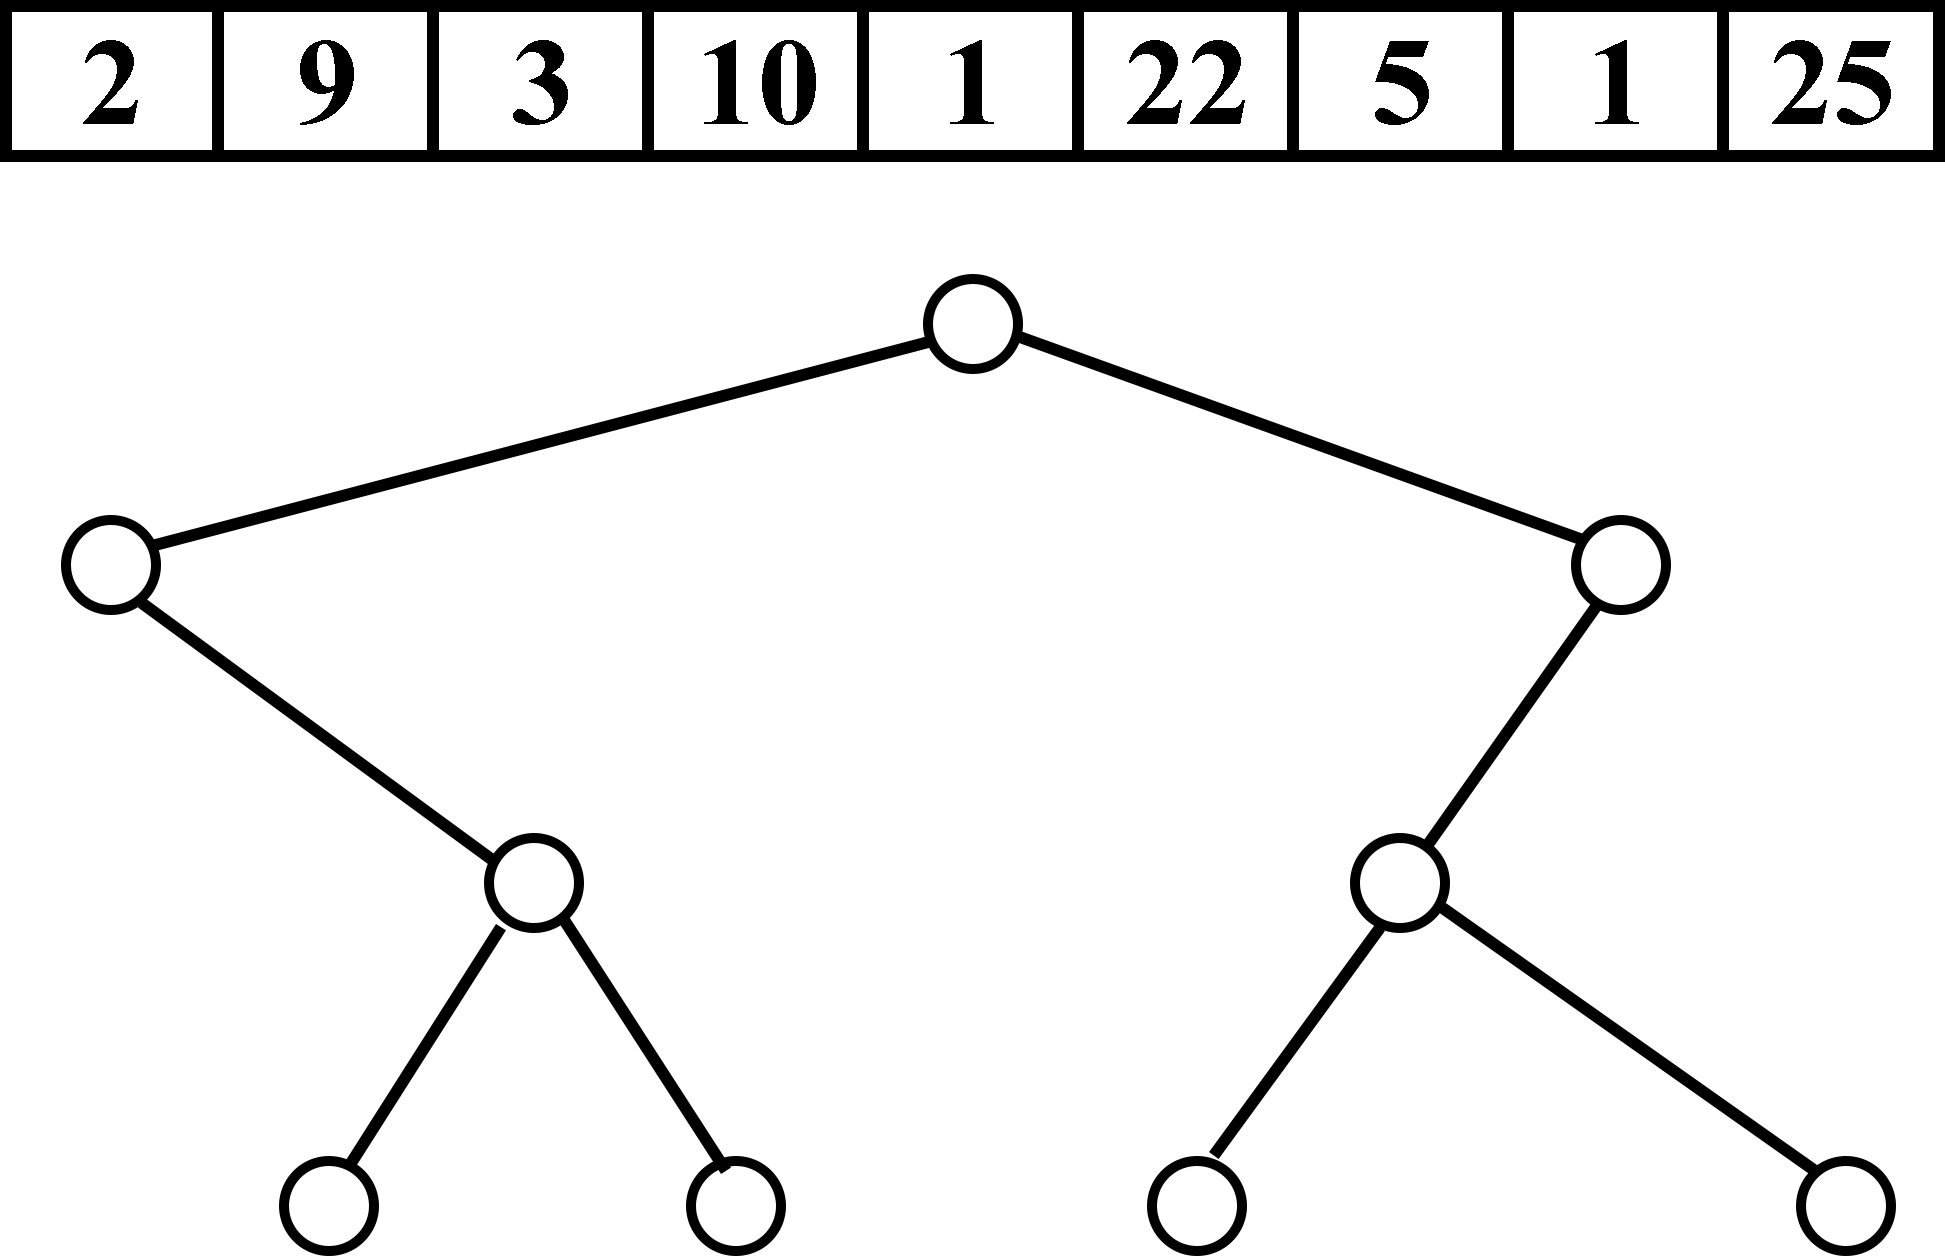
\includegraphics[width=0.6\textwidth]{pic/cartesian-tree-idea.png}
\caption{Пример декартова дерева}\label{fig:cartesian-idea}
\end{figure}

\revise{
Структура данных Декартового дерева позволяет очень простые алгоритмы, чтобы среднее время выполнения O (log n) для каждого из этих примитивов~\cite{cartesian-tree}. Декартовые дерево, построенные из 
последовательности различных чисел обладает следующими свойствами: Узлы в декартовой дереве соответствуют элементам в исходной последовательности, то есть каждый элемент в последовательности соответствует 
единственному узлу в дереве, каждый узел в дереве также соответствует единственному элементу в последовательности; С помощью метода обхода упорядоченную, исходная последовательность чисел может быть 
выведено, то есть, любой нижний индекс элемента из последовательности, представленной в левом поддереве дерева узла меньше, чем нижний индекс элемента из последовательности, представленной узлом, любой 
нижний индекс элемента из последовательности, представленной в правом поддереве дерева узла больше, чем нижний индекс элемента из последовательности, представленной узлом ; Структура данных Декартового 
дерева обладает тем же свойством, что и стек, то есть значение любого узла в дереве больше или меньше, чем значение любого узла из его левого или правого поддерева. По своему свойству типа стека, корневой 
узел является узлом с самым большим или наименьшим значением дерева, любой узел в дереве является узлом с самым большим или наименьшим значением поддерева, в том числе и себя.
}

\subsection{Параллельный алгоритм вычисления префиксных сумм}

\revise{
Алгоритм префикс сумма является одним из наиболее важных строительных блоков для расчета данных параллельных~\cite{sengupta06}. Оно было введено по~\cite{hillis86}. Для параллельных 
вычислений, данных параллельного стиль подходит для поддержки этого, алгоритм Приставка сумма составляет параллельно компьютеры контролируют параллельно стиль с помощью многопроцессорной
обработки~\cite{hillis86}. Работа алгоритма префикса сумма вычисления всех частичных сумм массива чисел. Эта концепция может быть описана с помощью простого выражения следующим образом.
}

\revise{
for j:=1 to log n do
    for all $k$ in parallel do
        if $k \ge 2^j$ then
            x[$k$] := x[$k - 2^(j-1)$] + x[$k$]
        fi
    od
od 
}

\revise{
Алгоритмы, которые могут использовать O (N) процессоров для вычисления операций с размером N, временная сложность алгоритма O (log n) время. На рисунке~\ref{fig:prefix-sum} показывает процедура 
интуитивного алгоритма префикса суммы.
}

\begin{figure}[!ht]
\centering
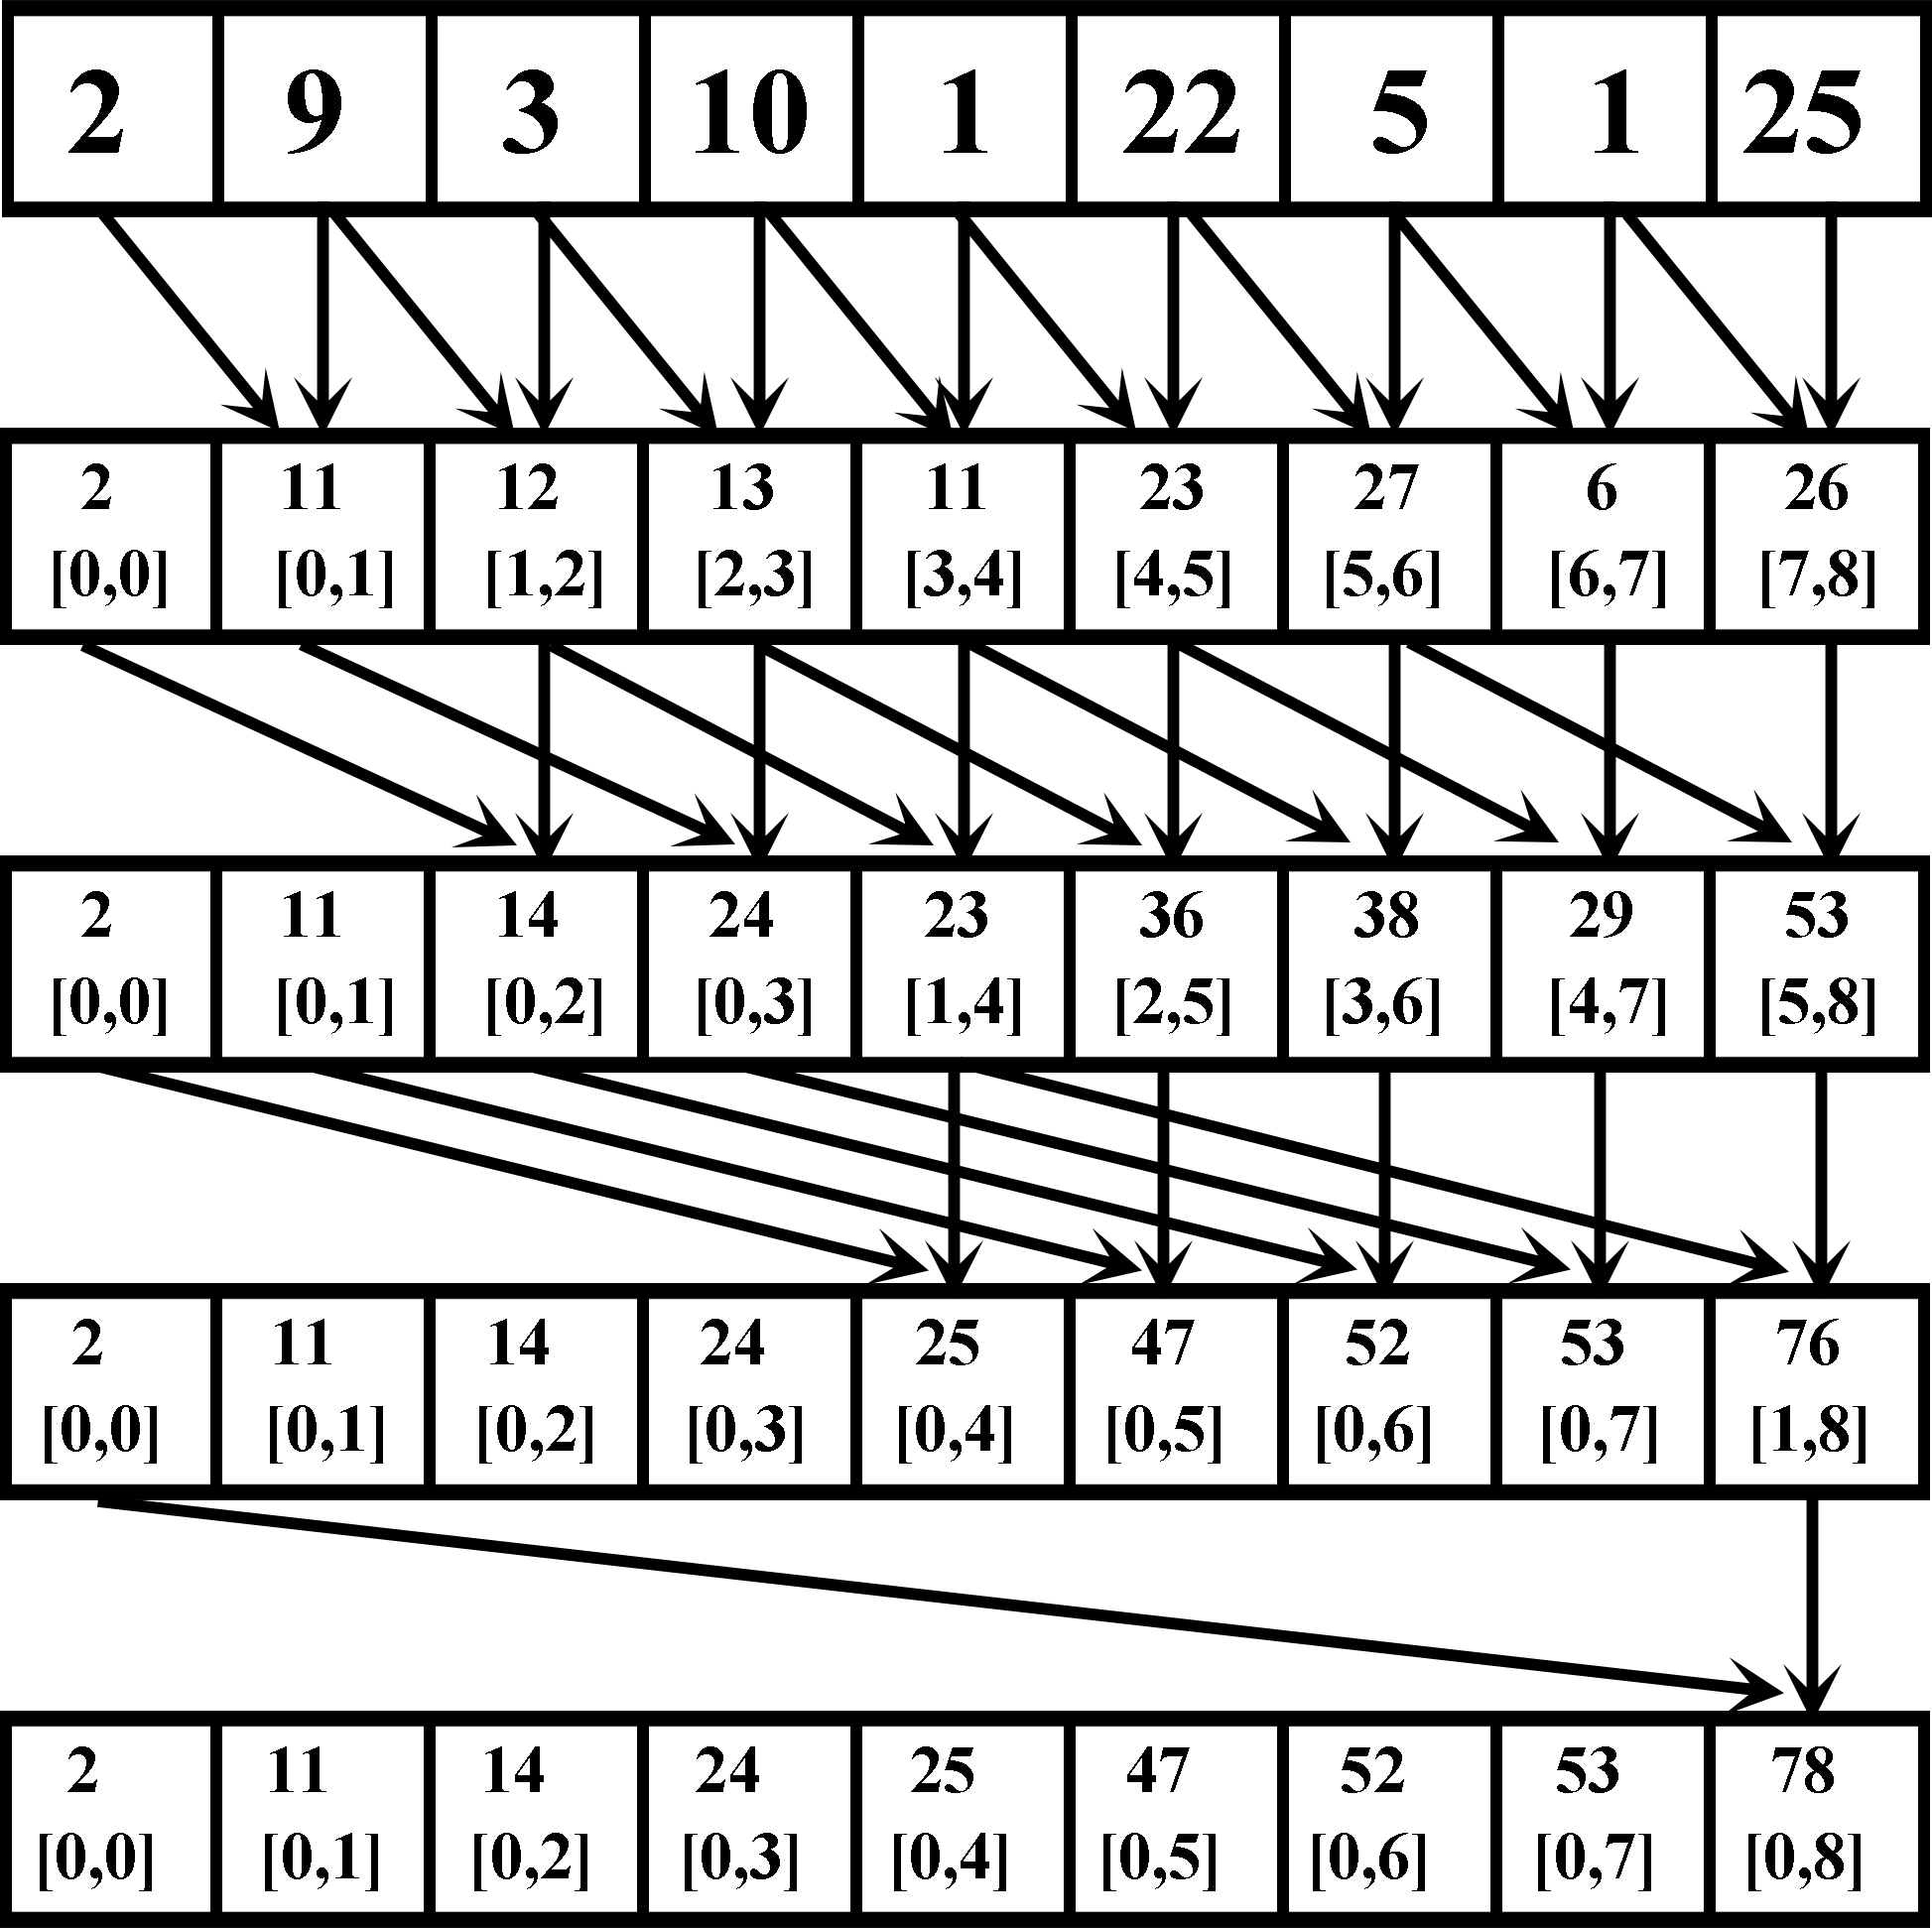
\includegraphics[width=0.7\textwidth]{pic/parallel-prefix-sum.png}
\caption{Иллюстрация идеи параллельного алгоритма вычисления префиксных сумм}\label{fig:prefix-sum}
\end{figure}

\chapterconclusion

\chapter{Постановка задачи}

\revise{
Проблемы исследования являются то, что структура данных могут быть использованы для достижения поставленных целей и какие ограничения существуют и каков алгоритм, основанный на структуре данных решении 
проблем динамического дерева. В результате обзора литературы, структура данных контракции параллельного дерева не достаточно для решения задач исследований, потому что необходима эффективная структура 
данных динамического дерева. Для того, чтобы ответить на динамические запросы и может быть продлен в параллельной обработки, эффективная динамическая структура данных дерева должна быть разработана. 
Сравниваемые динамические структуры данных дерева, RC-Trees имеют особенности, которые ST-Tree, Topology Tree и Top Tree имеют. RC-Trees улучшены по Acar U. et al. (2003) используют распространение 
изменения могут поддержать изменения в обновлении. В результате, структура данных RC-Trees подходит как базовая структура данных, используемая для покрытия дополнительных изменений в параллельной 
обработке.
}

\revise{
Особенностью RC-Trees требует дополнительного осуществления RC-Trees, Таким образом, первое улучшение должно сделать реализацию RC-Trees завершена. Во-вторых, структура данных RC-Trees нуждается в более 
технологически достижений программирования, чтобы сделать код пригодным для использования в современных приложениях. В-третьих, RC-Trees в параллельном процессе недостаточно эффективно, реализация должна 
сделать параллельный процесс в каждом граблями и сжать операции и между граблями и сжимают операций. Другими словами, в каждом вычислительном раунде, каждая операция лопаточки должна выполняться 
параллельно, так как при этом операции компресса. Тогда рейк и компресс операции должны выполняться параллельно.
}

\revise{
Кроме того, RC-Trees в теории в настоящее время, и структура не поддерживает данные некоммутативные типа, например, матрицы. Таким образом, в реализации и улучшения, эта функция должна быть добавлена, то 
лучше поддержать направленной и ненаправленной данные тоже. Структура данных должна работать эффективно и с простыми данными и больших объемов данных.
}

\section{Требования к реализации структуры данных}

\revise{
Проблемы исследования необходимо решить то, что структура данных могут быть использованы для достижения поставленных целей и какие ограничения существуют и каков алгоритм, основанный на структуре данных 
решения динамических задач дерева. В частности, выбранная структура данных должна поддерживать динамические запросы с постепенных изменений. Потому что следующая работа состоит в том, чтобы сделать 
структуру данных работу в параллельной обработке, поэтому поддерживают структуру, какие данные параллельных вычислений следует ответить. Тогда следующая проблема, если выбрана структура данных, алгоритм 
должен быть выбран так, чтобы сделать структуру данных работ. По сравнению с перечисленными структурой данных, RC-Tree cтруктура данных пригодна. Он поддерживает динамическое дерево и котракцию 
параллельного дерева. Он может решить проблемы, как правило, и RC-Tree cтруктура данных представлен по Acar. U. поддерживает изменения процессу обновления. RC-Trees реализовают алгоритм с котракции 
параллельным дерева, включая рейк и компресс операций. Распространение изменение делает поддержка дополнительных изменений возможно.
}

\revise{
Хотя первоначальная структура данных RC-Tree в основном отвечает требованиям решения задачи исследования, но он не поддерживает как коммутативные и некоммутативные данных. Кроме того, направленные ребра с 
информацией может получить сложно для вычислений. Сложность структуры данных ограничивает расширение для переключения на параллельных вычислений. Ограниченная степень RC-Tree поддерживает не все виды 
деревьев в лесу.
}

\revise{
В результате, RC-Trees не удовлетворяет, новая структура данных должна быть разработана на основе RC-Trees и должна поддерживать коммутативные и некоммутативные данных. Для того, чтобы избежать 
ограничения ограниченной степени, ассистент структура может быть использована для изменения исходного дерева в работоспособное и хранимого дерева. В следующих разделах, разработка новой структуры данных 
будет описана ниже.
}

\section{Интерфейс для запросов и модификаций}

\revise{
Новая структура данных, разрабатываемых в данной работе должны поддерживать динамические деревья, так что операции выполняются в лесу. В слое пользователя, корневое лес должен быть создан, вызывают каждый 
запросы основаны на этом лесу. В коренится лесу, есть корневые деревья, каждая вершина в лесу имеет корень. В частности, вершина, которая не имеет родителя является корнем. Как правило, в динамическом 
дереве, алгоритм в основном поддерживает запросы на получение номера вершин, ребер и корней в лесу. Кроме того, алгоритм поддерживает запросы на вершине с ответом число своих детей, возвращая его 
родителя, проверяя, если оно является корнем, получать информацию, которую она несет, или его ребра несут. Вершина несет информацию о себе, которая называется вершиной информации в этой диссертации, а 
также информацию о его ребер, которые соединяли между его родителями или детьми, которая называется ребро информация. Информация о вершина поддерживает коммутативную информацию и отвечает на запросы 
поддерево. Информация о ребре имеет две части, вверх информацию, которая направлена к родителю, а также информацию вниз, которая направлена от своих детей. Ребра могут нести гораздо больше информации, чем 
вершины, при этом ребра предназначены для поддержки как коммутативный и некоммутативную информации.
}

\revise{
При реализации алгоритма, существуют три основные интерфейсы поддерживаются отвечать на запросы о динамическом дереве, которые получают корень, получить путь и получить поддерево. Получить корневой 
интерфейс просто ищет родителя запроса вершины, если его родитель не является корнем, а затем продолжить поиски в прародителя запроса, тем, что аналогия, наконец, находит вершину, которая является корнем 
настоящего дерева, она занимает O (1) время. Интерфейс получить путь возвращает сводку информации по ребром на пути между двумя вершинами запроса. Очевидно, что только две вершины расположены в том же 
дереве путь между ними может быть найден. Для того, чтобы получить путь, если две вершины находятся в той же маленькой поддерева, что они просто нужно сделать, это один работает вниз и один работает, пока 
они не встретятся; если две вершины не в той же маленькой поддерева, они должны работать до самого низкого общего предка. Чтобы получить поддерево вершины запроса просто нужно добавить информацию о его 
поддерева и сама по себе. В RC-Tree, то ясно, что только вершина, которая не является корнем, который должен быть сжат имеет поддерево, поддерево информация вершины является сводной информации ее ребенка 
и поддерево от него ребенка.
}

\revise{
Чтобы ответить на динамические запросы более эффективным, механизм график здесь добавлен, который обновляет дерево в расписании. Каждый раз, когда некоторые изменения сделаны в лесу, он будет проверять, 
если изменения может быть сделано. Каждое изменение может быть записано, но если не делать применять расписание, изменения не будут внесены в лес. Операции, которые пользователи делают бы вызвать функцию 
расписания, что пользователи могут сделать, это сведения о параметрах вершину или ребро информацию о конкретной вершины, ребра между двумя вершинами могут быть подключены или удалены. Изменения, сделанные 
на дереве могут быть отменены или применены, функция отмены обновляет дерево, как и другие операции, то применять функцию выполнять все изменения, сделанные на дереве и, наконец, изменяет дерево. Эта 
функция график делает последующий параллельная работа более интуитивным и более удобным. Для ускорения времени вычислений при применении графика, параллельные операции выполняются в функции, когда 
применяется функция вызывает их.
}

\chapterconclusion

\chapter{Разработка структуры данных}

\section{Поддержка пользовательских типов пометок на вершинах и ребрах}

\section{Снятие ограничения на степень вершины}

\revise{
В этой диссертации, если предположить, что в лесу каждая вершина имеет не более трех детей. Поскольку установка ограниченной степени для более простой оценки, в бинарном дереве каждая вершина имеет не 
более двух детей, третий ребенок установлен здесь используется для внутренней структуры данных для выполнения вычислений.
}

\revise{
Пользователи могут создавать любые деревья, они хотят, делают динамическое дерево не может быть бинарное дерево. В этой диссертации, с использованием внутреннего дерева - декартово дерево, чтобы сохранить 
фактические данные. Когда график операция присоединения выполнена, она вызывает декартово дерево, чтобы соединить две вершины, и в декартовой дереве, индекс вершины не то же самое, как и в представленном 
дереве, информация ребро будет храниться в детской вершины в тип данных вершин. Например, пользователи вершинные выполненном V, в декартовой дереве, она хранится в виде 2*V, в результате, вершина в 
декартовой дерева не делает влияния на вершине в представленном дереве, но содержит информацию от него. Ребенок вершина в представленном дереве будет располагаться в поддереве его родителя в декартовой 
дереве. Каждое изменение в представленном дереве, такие как вложение, отслоение и информацию о наборе вершин будем называть декартово дерево, чтобы обновить изменения фактического сохраненного дерева.
}

Основной проблемой имеющихся реализаций является константное ограничение на максимальную степень вершины~\cite{acar04}. В настоящей работе его предлагается преодолевать
с помощью следующего приема. Каждая вершина оригинального дерева разбивается на две вершины~--- \emph{вершину данных} (или <<нижнюю>> вершину) и \emph{вершину связей} (или <<верхнюю>> вершину).
Вершина данных всегда имеет родителем соответствующую вершину связей. При этом все дети той или иной вершины организуются в двоичное дерево поиска, корнем которого служит вершина данных родителя, а
остальными вершинами~--- вершины связей детей. В качестве двоичного дерева поиска использовалось декартово дерево~\cite{cartesian-tree}. При таком подходе степень каждой вершины не превосходит трех, что
позволяет использовать алгоритмы для вершин с константной степенью. На рисунке~\ref{fig:represented} приведено оригинальное дерево и дерево, получающееся путем удвоения вершин и организации детей каждой
вершины в виде дерева.

Каждая вершина оригинального дерева снабжена меткой, тип которой является коммутативным моноидом, при этом структура данных поддерживает операцию <<вычислить моноидную сумму меток всех вершин в поддереве
данной вершины>>. Аналогично, каждое ребро оригинального дерева снабжено двумя метками (метка, соответствующая направлению от ребенка к родителю, или <<вверх>>, и аналогичная метка <<вниз>>),
тип которых совпадает и является моноидом (возможно, некоммутативным), при этом структура данных поддерживает операцию <<вычислить моноидную сумма меток всех ребер на пути от вершины $A$
к вершине $B$ для данных вершин $A$ и $B$>>. При удвоении вершин, метки вершин и ребер, выходящих вверх из вершин оригинального дерева, переходят в соответствующие метки соответствущих вершин данных,
в то время как метки вершин и выходящих вверх ребер у вершин связей равны нейтральным элементам соответствующих моноидов. Таким способом достигается корректность выполнения запросов независимо от
структуры деревьев, организующих детей вершин.

\begin{figure}[!ht]
\centering
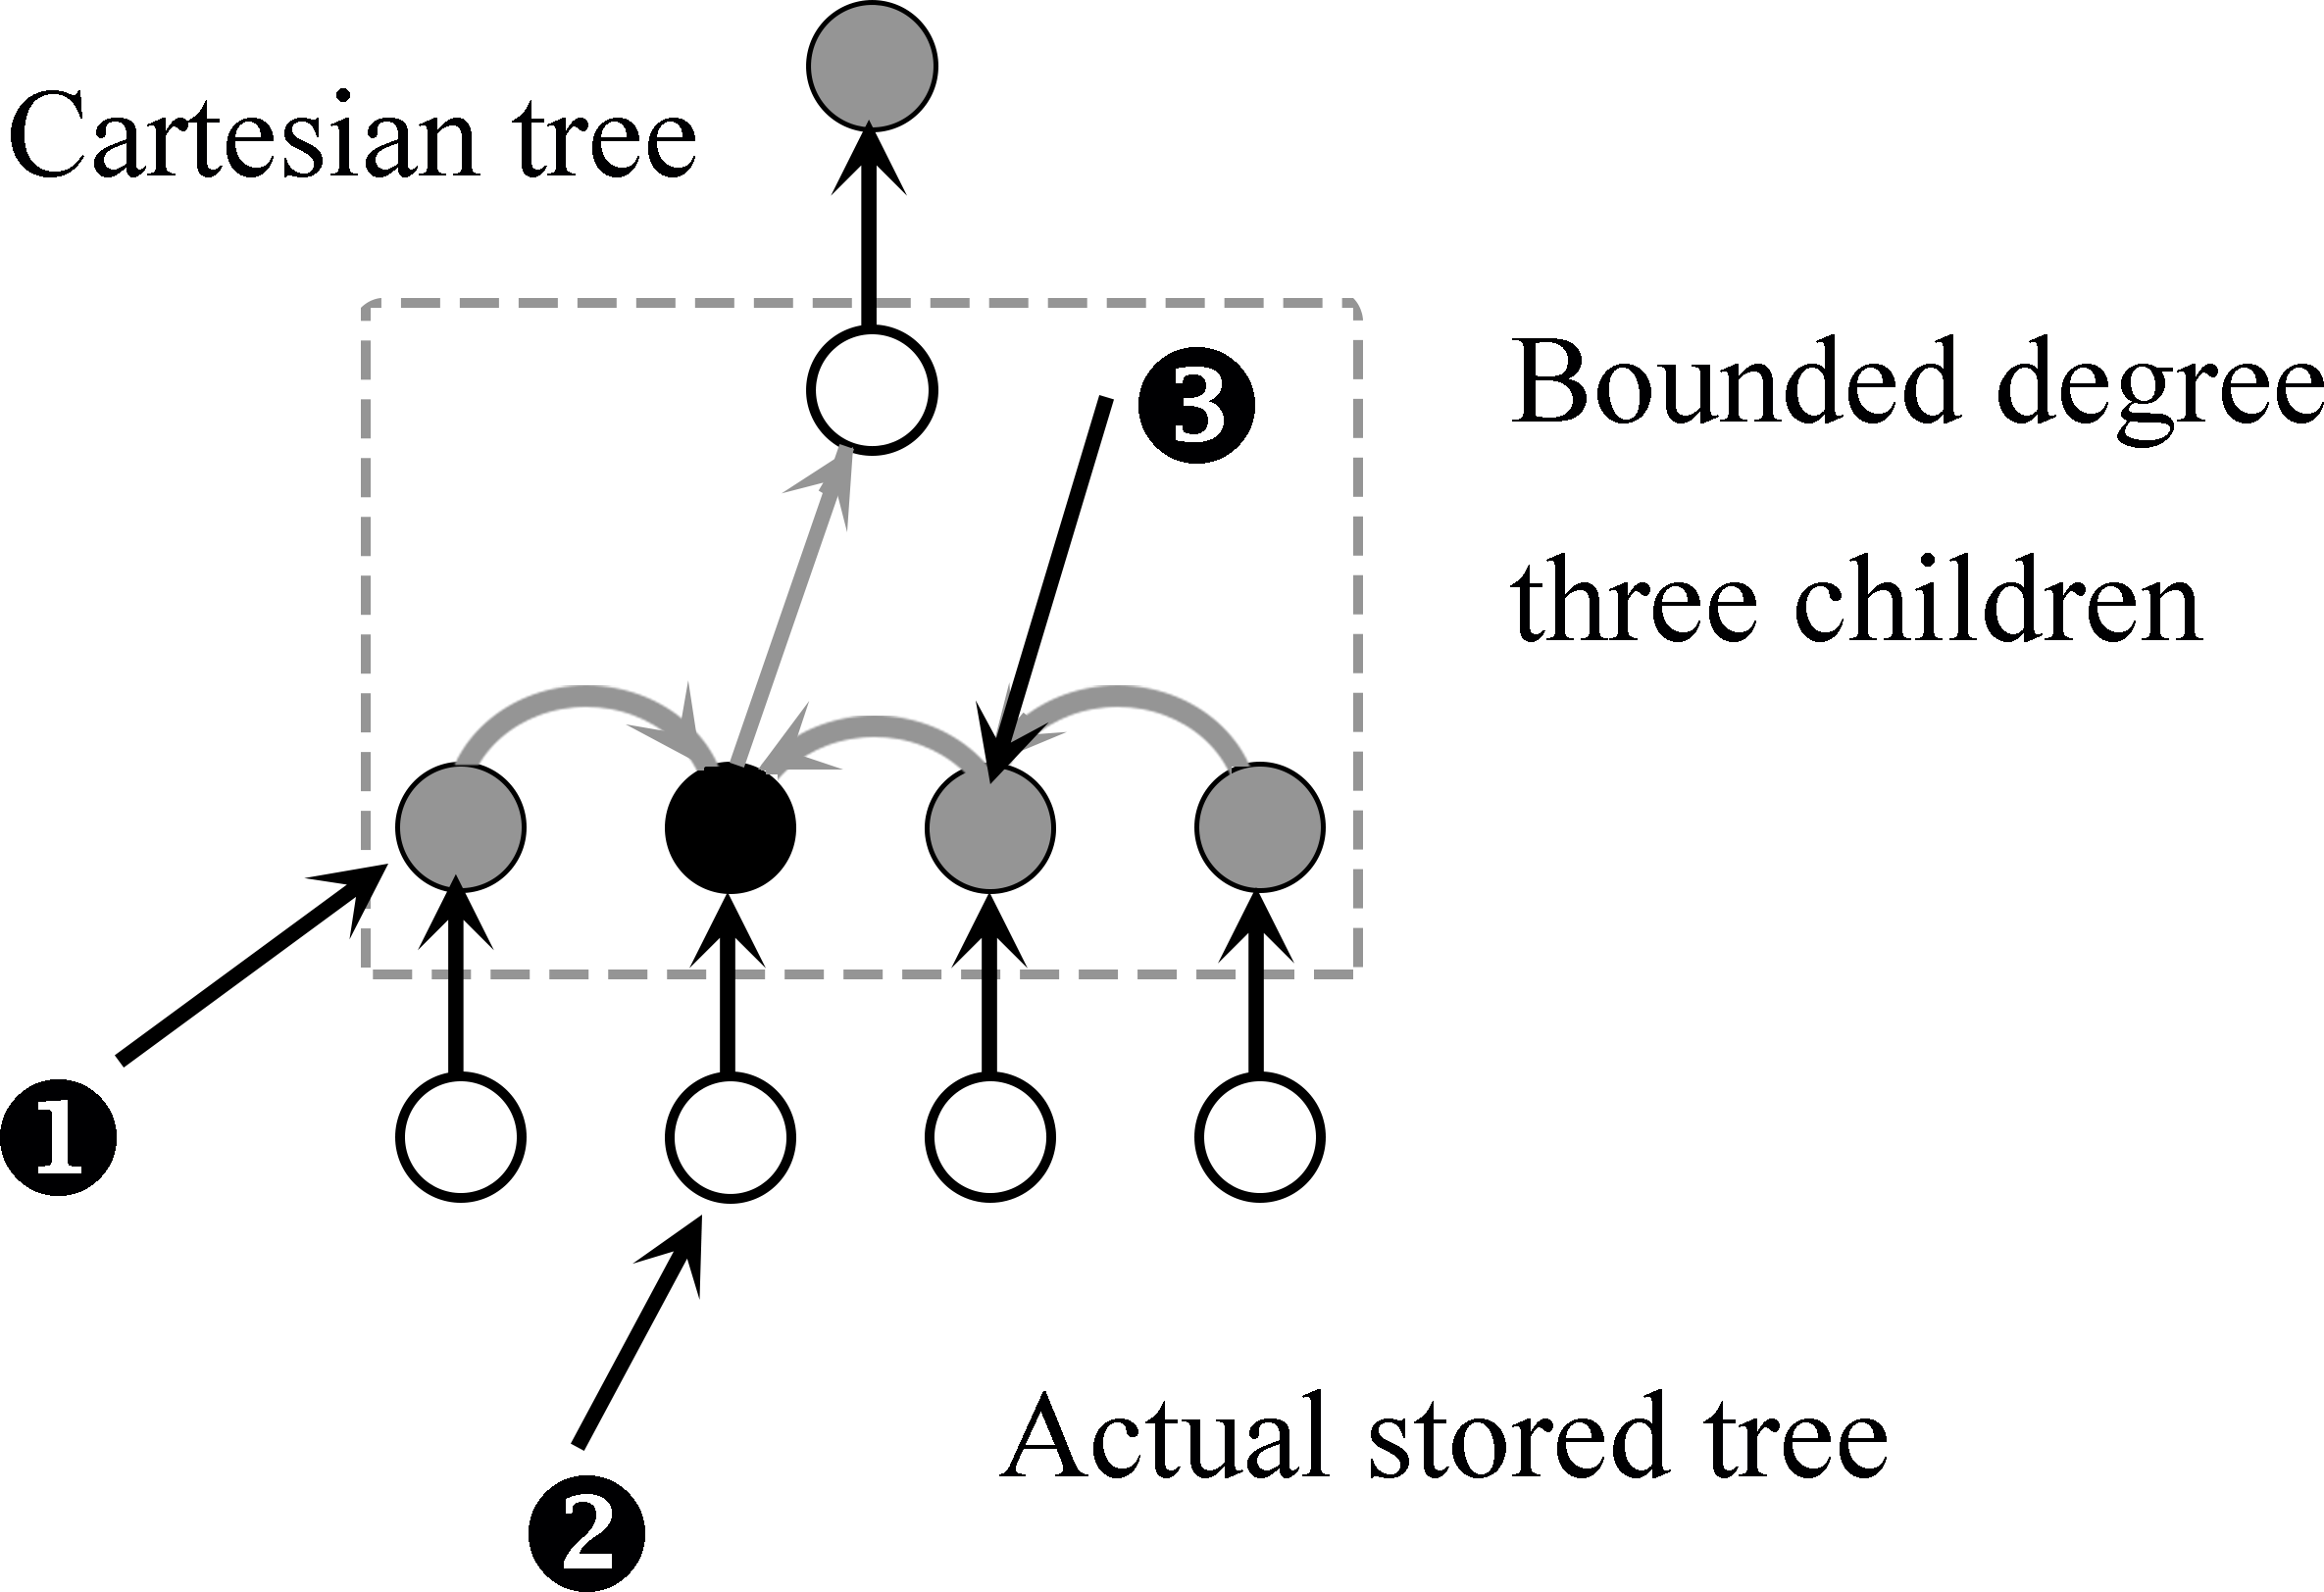
\includegraphics[width=0.55\textwidth]{pic/Cartesian_tree.png}
\caption{Представление вершины и ее детей с помощью декартова дерева}\label{fig:cartesian-children}
\end{figure}

\begin{figure}[!ht]
\centering
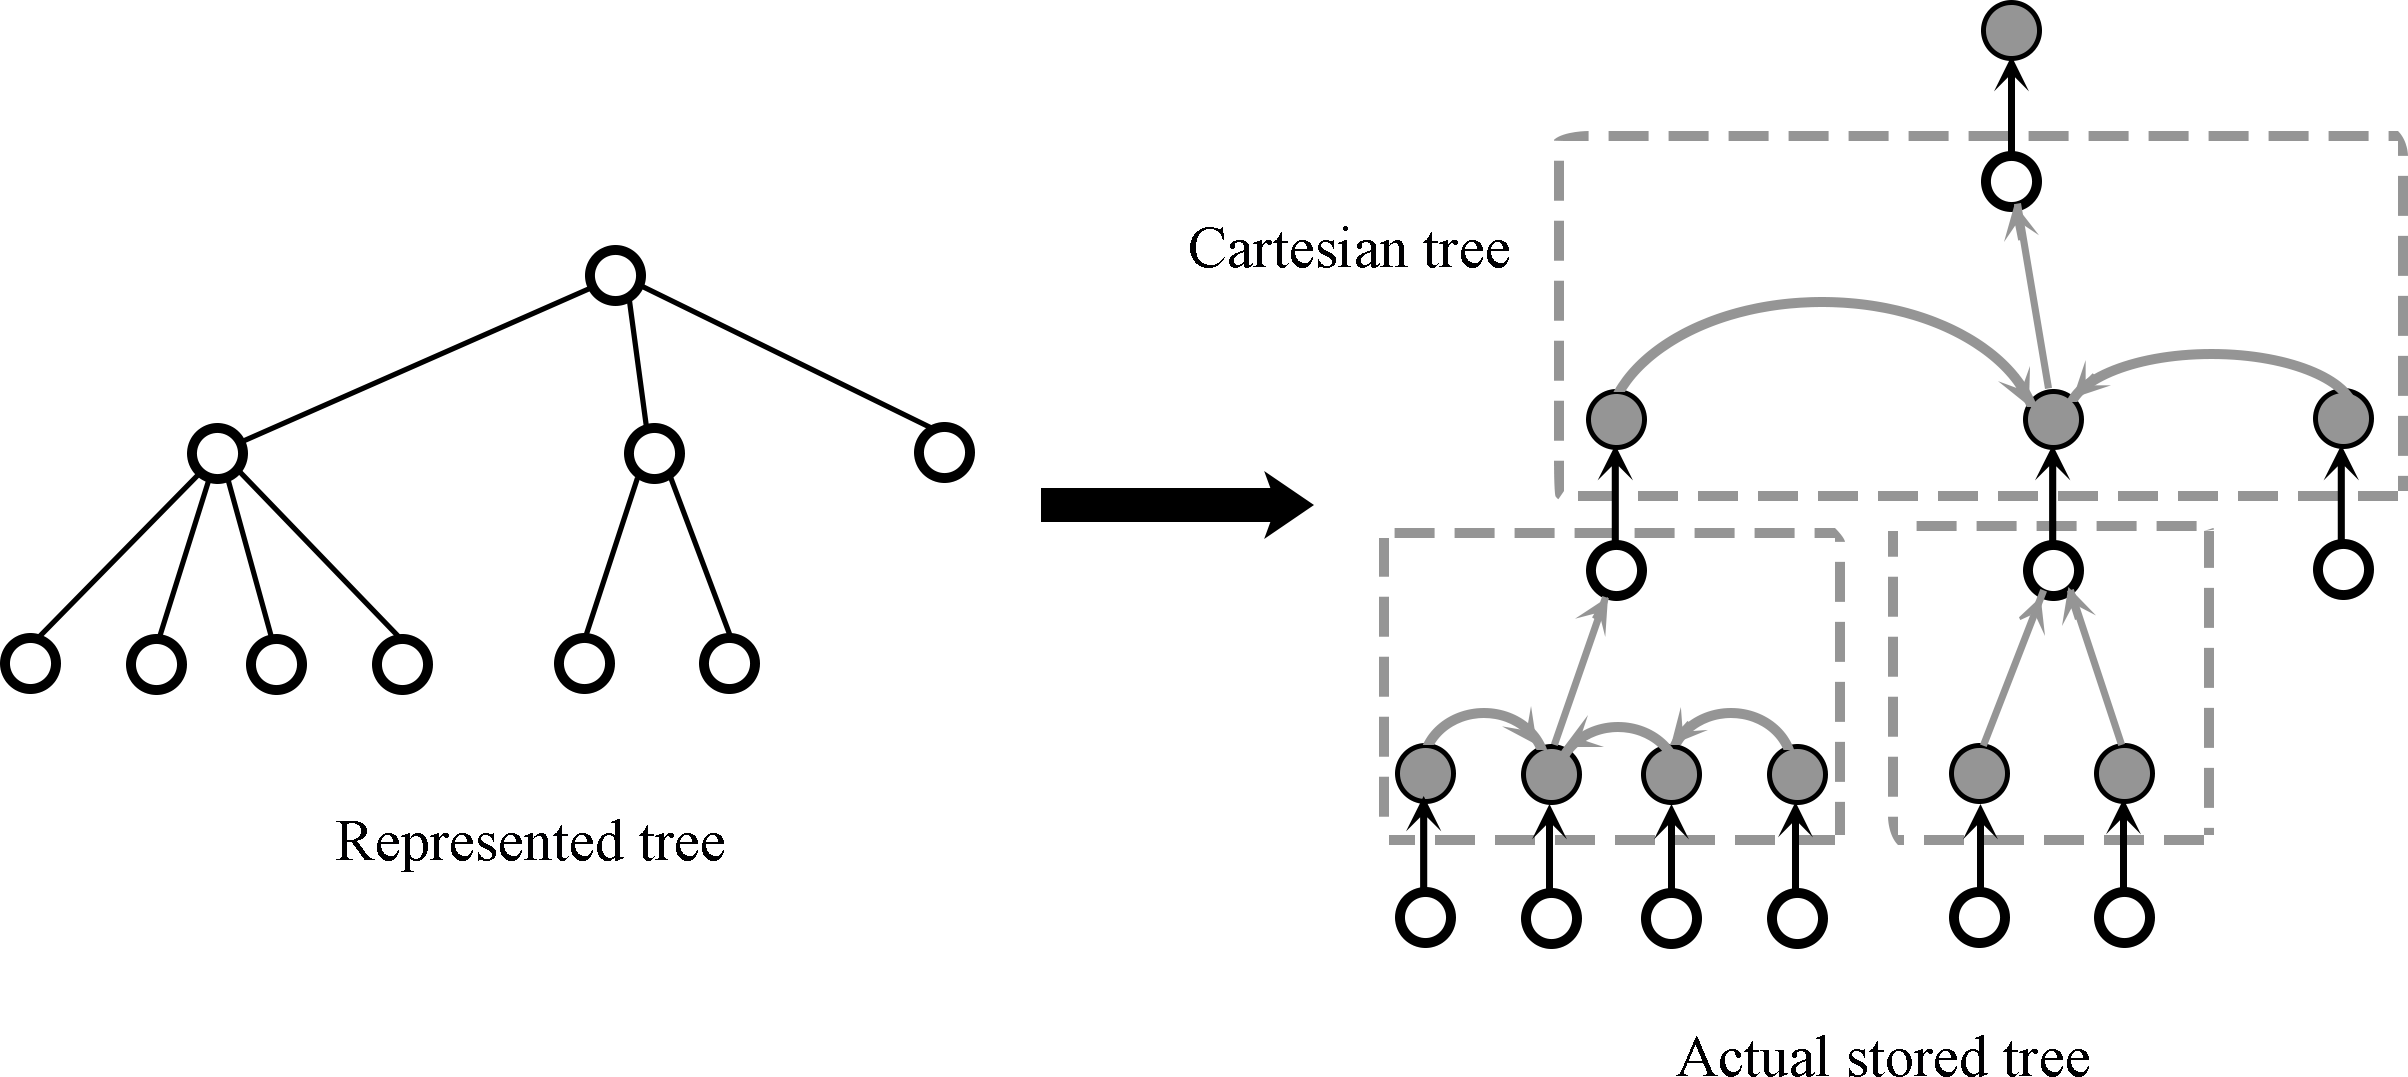
\includegraphics[width=1.0\textwidth]{pic/represented_tree_and_actual_stored_tree.png}
\caption{Исходное RC-дерево и дерево, которое хранится в памяти}\label{fig:represented}
\end{figure}

%Исходный код реализации дерева, а также нижеследующих экспериментов, располагается в репозитории GitHub по адресу
%\url{https://github.com/feng7/pasl/tree/pdt/example/rc-tree}.

\section{Хранение данных в $O(N)$ оперативной памяти}

\revise{
Структура данных разработана в диссертации, которая поддерживает операции динамических изменений. Как используется механизм расписания, в структуре данных, уровни используются для разъяснения операций. 
Тогда каждая вершина имеет тип вершин столбец, который записывает в вершине каждый раз, когда она изменяется, как показано на рисунке. Все новые созданные вершины на первом уровне в структуре, как только 
они меняются, они выталкиваются на следующий уровень, это выглядит как 2-й матрице. Вершины типа столбца имеют свою информацию об уровне. В результате, в расписании просто проверить последний живой 
уровень, где вершина может делать операции правильно.
}

\begin{figure}[!ht]
\centering
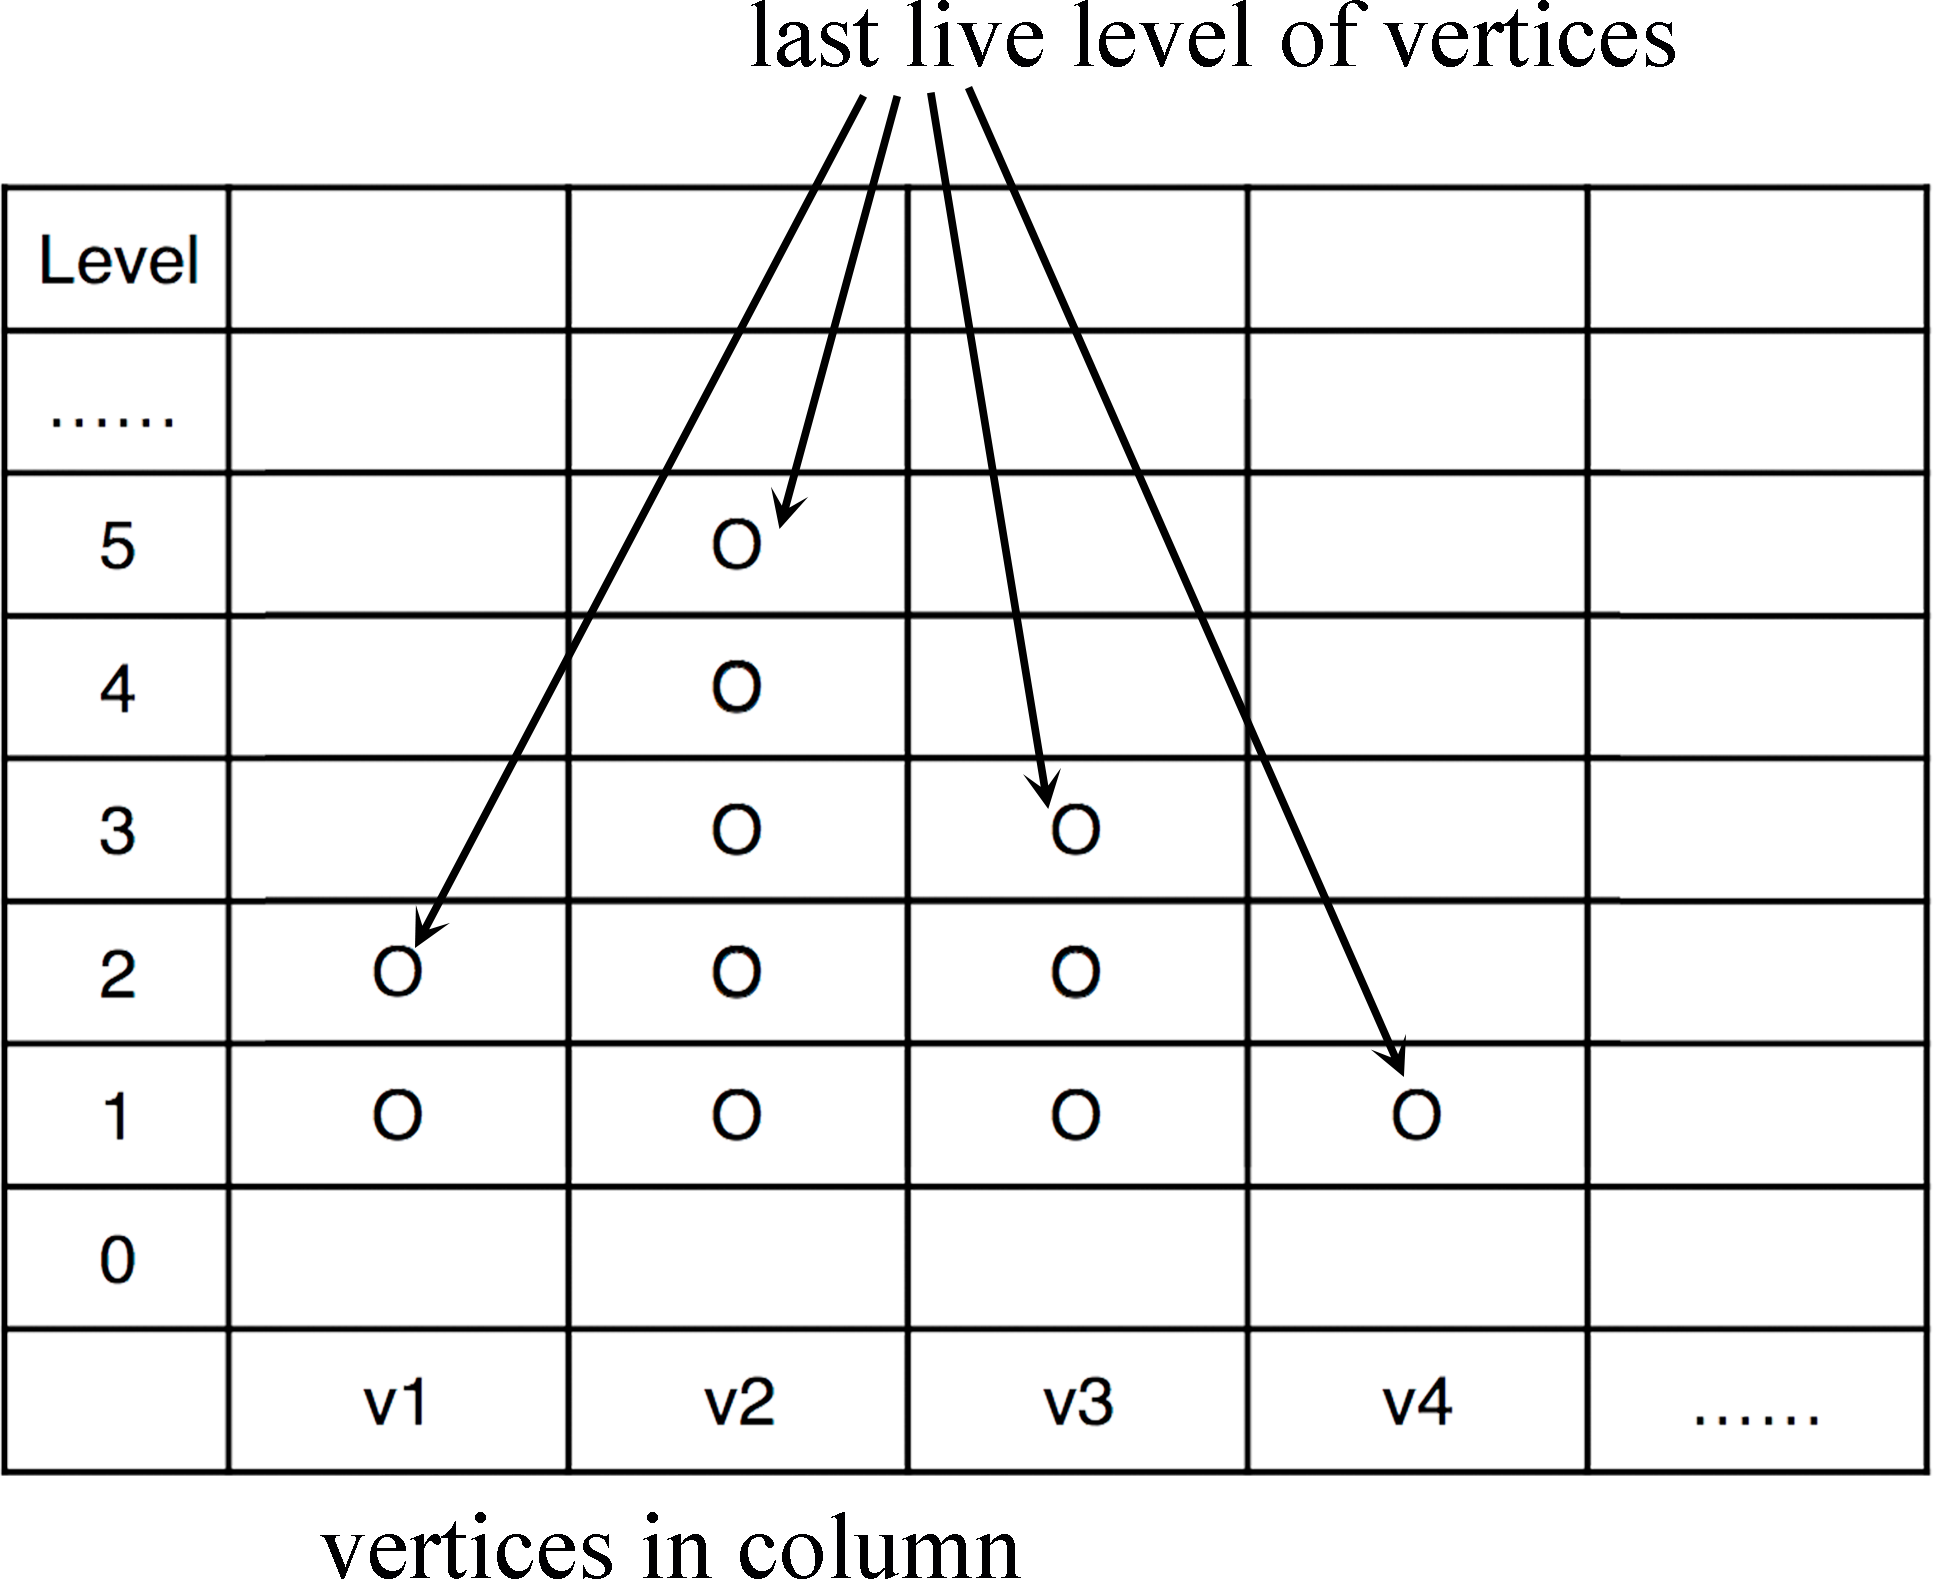
\includegraphics[width=0.7\textwidth]{pic/vertices_in_column.png}
\caption{Хранение данных в $O(N)$ оперативной памяти}\label{fig:memory}
\end{figure}

\section{Проверка применимости модификаций}

\revise{
Для того, чтобы избежать ошибочных операций, сделанные на дереве, в этой диссертации, проверка ошибок интерфейс создается для проверка ошибок называется динамической связи. Как правило, операции, 
выполняемые на динамическом дереве с двумя вершинами требуют проверки их отношений. В динамической связи, проверка связи и проверка соединения между двумя вершинами проверить, если они связаны между собой 
или в том же дереве. Она занимает O (log n) времени каждый раз, когда операция обновления спрашивается, однако это не является необходимым, чтобы сделать ошибку проверки каждый раз, когда, например, когда 
операция открепление просят, только чтобы проверить, если вершина является корнем необходимо, в операции среза будет проверять степень первой вершины, потому что только тогда, когда вторая вершина 
является ее ребенок операция может быть сделано верно. Таким образом, проверка ошибка во время операции срезали O (log n) до O (log d), где d является степень родителя.
}

\section{Применение обновлений}

\revise{
Как уже упоминалось выше, уровни используются для обозначения модифицированный вершин, каждый из которых работает круглый. Когда операция применяется называется, положить последние эксплуатируемые вершины 
от уровня 0 до уровня 1. Затем сделайте петлю, чтобы применить операции на каждом уровне, в соответствии с количеством модифицированных вершин, функция процесса вершина называется. Функция проверяет 
состояние вершины, если текущая вершина является последней живая вершина в его колонке, то функция будет просто сделать рейк или компрессия или другие изменения непосредственно, если текущая вершина не 
живая вершина, вызов функции для себя и толкать текущую вершину на следующий уровень. В другом слове, функция делает фактическую работу по обновлению динамического дерева. После того, как функции процесса 
вершины на том же уровне, необходимо проверить количество своих следующих затрагиваемых вершин, чтобы получить новые числа следующих затрагиваемых вершин текущей вершины на следующем уровне.
}

\revise{
В функции процесса вершины, до того, как применяется сделаны, вершины должны быть проверены, если бы операцию. В \texttt{will{\textunderscore}*} процедуры в функции будет проверять, если вершина станет 
корнем, или будет сгребают, 
или будут сжаты, или будут иметь изменения, но может быть сделать рейк или компрессия на следующем уровне. Если результат проверки верно, то \texttt{do{\textunderscore}*} операции выполняют работу. Если 
вершина сгребают, 
это будет влиять на его родителей, и число его следующих затрагиваемых вершин должны плюс один. Если вершина сжимается, она будет влиять как на его родителей и детей, как уже упоминалось выше, фактическое 
хранится дерево использует декартово дерево, затронутый ребенок будет только ее первый ребенок. В других случаях, вызовите функцию процесса изменили вершину на следующем уровне.
}

\section{Реализация параллельных вычислений}

\revise{
Когда была разработана структура данных, она работает в очередной раз уже. Как уже упоминалось выше, параллельное вычисление будет сделано в цикле с помощью вызова функции процесса вершинный в расписании 
применить операцию. Функция применяется работает в цикле уровней, чтобы проверить все измененные или пораженные вершины. Параллельные вычисления будут работать на каждом уровне для каждой вершины, в 
результате, в новом алгоритме, разработанном в данной работе, на каждом уровне, операции рейк, операции компресс, поворот к корневой операции, а также другие необходимые операции выполняются параллельно, 
когда они находятся на том же уровне. Результат каждого вычисления уровня будет влиять на его следующий уровень, было бы лучше, чтобы не выполнять функции каждого уровня параллельно.
}

\revise{
Циклические драйверы используются в структуре данных, это облегчает для переключения параллельных методов. В функции применяются, измените функцию контура для функции водителя, а функция Compute prefix 
sum, а также. Для сравнения, зацикливание драйвер выполняет в последовательном использует функцию общего цикла.
}

\chapterconclusion

\chapter{Экспериментальное исследование}

\revise{
Алгоритм разработан и внедрен выше, в этой части, есть три случая, чтобы оценить его эффективность. Последовательное время как раз оценивается в качестве основного стандарта для сравнения параллельной 
работы. В параллельной обработки данных, используются две библиотеки, в PASL и OpenMP будет сравнивать друг с другом. Испытательная машина имеет 4 ядра процессора и 4 Гб памяти.
}

\section{Тестовые сценарии}

Эксперименты по измерению времени построения разработанной реализации и выполнения ею запросов производятся на следующих тестах:
\begin{enumerate}
    \item дерево-<<палка>>: $n$ вершин, при этом $i$-тая вершина является ребенком $(i-1)$-ой вершины при $i > 0$.
    \item дерево-<<пучок>>: $n$ вершин, при этом $i$-тая вершина является ребенком вершины 0 при $i > 0$.
    \item дерево-<<два пучка>>: $n$ вершин при $n = 2m$, $m$ целое, при этом вершина 0 является родителем вершин с 1 по $(m-1)$,
          вершина $m$ является родителем вершин с $(m+1)$ по $(n-1)$, а вершины 0 и $m$ дополнительно соединены.
    \item построение дерева-<<палки>> в десять этапов, каждый из которых состоит в присоединении $n / 10$ вершин.
\end{enumerate}

\section{Экспериментальное исследование последовательной реализации}

\revise{
Проще говоря, сделаны там четыре испытания: во-первых, построить n вершин линейного дерева, которая называется длинной цепью; во-вторых, построить n вершины стека, называется большой степени; в-третьих, 
построить два штабеля с n вершинами, которые называются два больших степеней; в-четвертых, построить дерево палку с десятью этапов, каждый из которых соединены n/10 вершин, называемых инкрементный длинной 
цепью. Число вершин будут назначены разные значения. Каждый раз, после того, как построение дерева п вершин, есть также n поддерево запросы к и n запросов пути, проведенные. В таблице приведены 
эксплуатационные времена структуры данных на тестах. Средняя сложность алгоритма является O (log n).
}

\begin{table}[!ht]
\centering
\begin{tabular}{|l|l|l|l|l|}\hline
 & $n=10000$ & $n=100000$ & $n=1000000$ & $n=2000000$ \\\hline
1 long chain & 0.089071 & 0.911241 & 9.85278 & 20.318 \\\hline
2 large degree & 0.045972 & 0.497738 & 4.75734 & 9.60901 \\\hline
3 two large degrees & 0.050595 & 0.506037 & 4.97508 & 9.7628 \\\hline
4 incremental long chain & 0.076277 & 0.980453 & 9.67115 & 19.5424 \\\hline
\end{tabular}
\caption{Результаты экспериментов для последовательной реализации}\label{tbl:results-seq}
\end{table}

\section{Экспериментальное исследование реализации с использованием OpenMP}

\revise{
Тестовые эксперименты здесь OpenMP используется для проверки параллельного времени работы. Тестовые такие же, как и в последовательном испытании. Тем не менее, OpenMP может использовать изменяемые 
процессоров в вычислительной машине. Там тесты, чтобы проверить эффективность OpenMP с числа процессоров 1, 2, 4, 8 и 16.
}

\revise{
Параллельный метод с использованием OpenMP применяется в зацикливание драйвер. Для общей для цикла, добавив заявление выше выражения цикла 
\texttt{\#pragma omp parallel for schedule (guided, 100)}. В этом 
эксперименте, размер резьбовом планирования заданий устанавливается с помощью управляемой 100. Каждый поток вычисляет минимальный размер в 100 раз петли. Для функции compute prefix sum, сначала вычислить 
частичное резюме параллельно; во-вторых, проверьте, если достигнут конец цикла и следующий цикл начинают непрерывно, чтобы убедиться, что результат от параллельных вычислений правильно, то проверка 
выполняется в одном потоке. Таблицы показывают операцию, приуроченный с помощью OpenMP.
}

\begin{table}[!ht]
\centering
\begin{tabular}{|l|l|l|l|l|}\hline
 & $n=10000$ & $n=100000$ & $n=1000000$ & $n=2000000$ \\\hline
1 long chain & 0.121935 & 1.01198 & 9.55426 & 18.5336 \\\hline
2 large degree & 0.049391 & 0.508561 & 4.90871 & 9.92507 \\\hline
3 two large degrees & 0.049772 & 0.526611 & 5.08418 & 10.1533 \\\hline
4 incremental long chain & 0.079227 & 1.02531 & 10.0432 & 19.9904 \\\hline
\end{tabular}
\caption{Результаты экспериментов для OpenMP, один процессор}\label{tbl:results-openmp-1}
\end{table}

\begin{table}[!ht]
\centering
\begin{tabular}{|l|l|l|l|l|}\hline
 & $n=10000$ & $n=100000$ & $n=1000000$ & $n=2000000$ \\\hline
1 long chain & 0.126611 & 1.17793 & 11.4037 & 21.5946 \\\hline
2 large degree & 0.050046 & 0.546854 & 5.32824 & 10.9253 \\\hline
3 two large degrees & 0.049792 & 0.57139 & 5.47457 & 10.9408 \\\hline
4 incremental long chain & 0.170487 & 1.29288 & 11.9869 & 23.686 \\\hline
\end{tabular}
\caption{Результаты экспериментов для OpenMP, два процессора}\label{tbl:results-openmp-2}
\end{table}

\begin{table}[!ht]
\centering
\begin{tabular}{|l|l|l|l|l|}\hline
 & $n=10000$ & $n=100000$ & $n=1000000$ & $n=2000000$ \\\hline
1 long chain & 0.155524 & 1.43204 & 13.5562 & 28.4551 \\\hline
2 large degree & 0.061891 & 0.630946 & 6.16235 & 12.615 \\\hline
3 two large degrees & 0.067719 & 0.660055 & 6.43371 & 12.7257 \\\hline
4 incremental long chain & 0.257657 & 1.70981 & 15.3224 & 31.0651 \\\hline
\end{tabular}
\caption{Результаты экспериментов для OpenMP, четыре процессора}\label{tbl:results-openmp-4}
\end{table}

\section{Экспериментальное исследование реализации с использованием PASL}

\revise{
Тестовые эксперименты здесь похожи с тестированием OpenMP, в этой части, изменяемые процессоры тестируются. Параллельный метод с использованием PASL применяется в pasl водителя по замкнутому кругу. Для 
общей для петли, с помощью простого оператора для параллельно для выражения цикла \texttt{pasl::sched::native::parallel{\textunderscore}for}. Для функции compute prefix sum, сначала вычислить частичное 
резюме параллельно; 
во-вторых, два делают цикл непрерывно, чтобы убедиться, что результат от параллельных вычислений является правильным. Таблицы показывают время срабатывания при использовании PASL с различным числом 
процессоров.
}

\begin{table}[!ht]
\centering
\begin{tabular}{|l|l|l|l|l|}\hline
 & $n=10000$ & $n=100000$ & $n=1000000$ & $n=2000000$ \\\hline
1 long chain & 0.12811 & 1.06817 & 10.4488 & 21.3671 \\\hline
2 large degree & 0.048464 & 0.542709 & 5.29652 & 10.7423 \\\hline
3 two large degrees & 0.050277 & 0.572261 & 5.41797 & 11.1019 \\\hline
4 incremental long chain & 0.083549 & 1.03886 & 10.654 & 21.7619 \\\hline
\end{tabular}
\caption{Результаты экспериментов для PASL, один процессор}\label{tbl:results-pasl-1}
\end{table}

\begin{table}[!ht]
\centering
\begin{tabular}{|l|l|l|l|l|}\hline
 & $n=10000$ & $n=100000$ & $n=1000000$ & $n=2000000$ \\\hline
1 long chain & 0.21437 & 1.84844 & 17.2076 & 34.3466 \\\hline
2 large degree & 0.139132 & 1.1316 & 10.7118 & 22.7569 \\\hline
3 two large degrees & 0.138923 & 1.14019 & 11.0991 & 22.452 \\\hline
4 incremental long chain & 0.204059 & 2.026 & 18.2874 & 39.5891 \\\hline
\end{tabular}
\caption{Результаты экспериментов для PASL, два процессора}\label{tbl:results-pasl-2}
\end{table}

\begin{table}[!ht]
\centering
\begin{tabular}{|l|l|l|l|l|}\hline
 & $n=10000$ & $n=100000$ & $n=1000000$ & $n=2000000$ \\\hline
1 long chain & 0.449078 & 4.67968 & 34.6637 & 70.9654 \\\hline
2 large degree & 0.287824 & 2.90302 & 24.2342 & 50.4066 \\\hline
3 two large degrees & 0.293782 & 2.6783 & 24.3486 & 48.1919 \\\hline
4 incremental long chain & 0.463437 & 4.70191 & 36.951 & 73.8718 \\\hline
\end{tabular}
\caption{Результаты экспериментов для PASL, четыре процессора}\label{tbl:results-pasl-4}
\end{table}

\section{Сравнение результатов экспериментов}

\revise{
Последовательный эксперимент выполняется в одном потоке. На рисунке показано сравнение времени наработки между последовательным, OpenMP и PASL. Другие две цифры показывают сравнение действующих раз с 2-х 
и 4-х процессоров между OpenMP и PASL.
}

\begin{figure}[!ht]
\centering
\begin{subfigure}[b]{0.45\textwidth}
    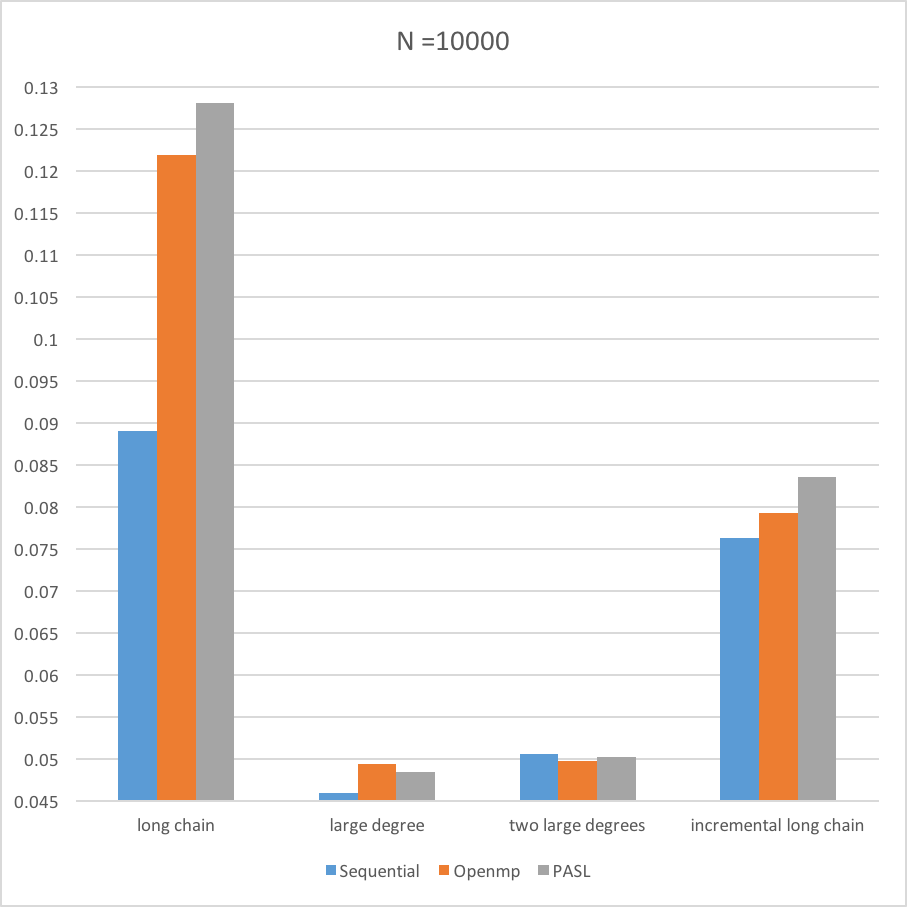
\includegraphics[width=\textwidth]{pic/results-1-a.png}
\end{subfigure}~~\begin{subfigure}[b]{0.45\textwidth}
    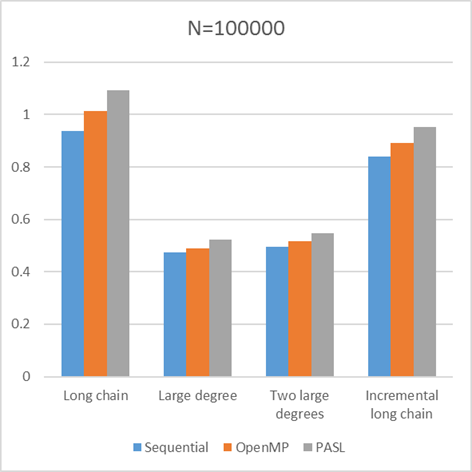
\includegraphics[width=\textwidth]{pic/results-1-b.png}
\end{subfigure}\\
\begin{subfigure}[b]{0.45\textwidth}
    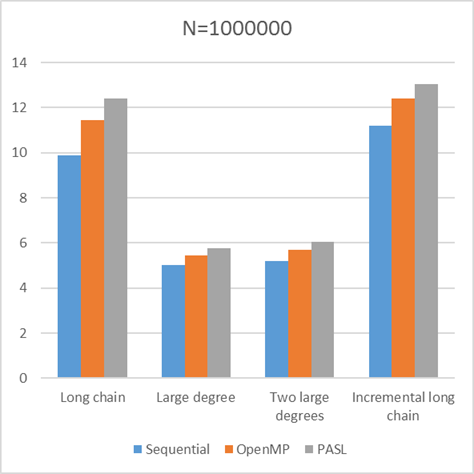
\includegraphics[width=\textwidth]{pic/results-1-c.png}
\end{subfigure}~~\begin{subfigure}[b]{0.45\textwidth}
    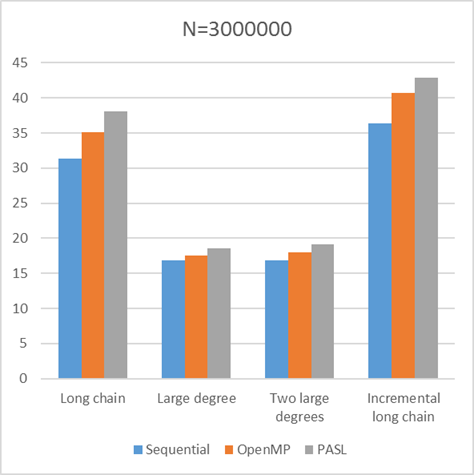
\includegraphics[width=\textwidth]{pic/results-1-d.png}
\end{subfigure}
\caption{Сравнение результатов, один процессор}\label{fig:results-comparison-1}
\end{figure}

\revise{
На рисунке, высота время каждая операция выполняется, из рисунка в общем, последовательное вычисление является наилучшим. Кроме того, можно видеть, что в большом линейном вычислением как длинной цепи, то 
OpenMP не занимает меньше времени. В целом, PASL может занять много времени, только на одном процессоре.
}

\begin{figure}[!ht]
\centering
\begin{subfigure}[b]{0.45\textwidth}
    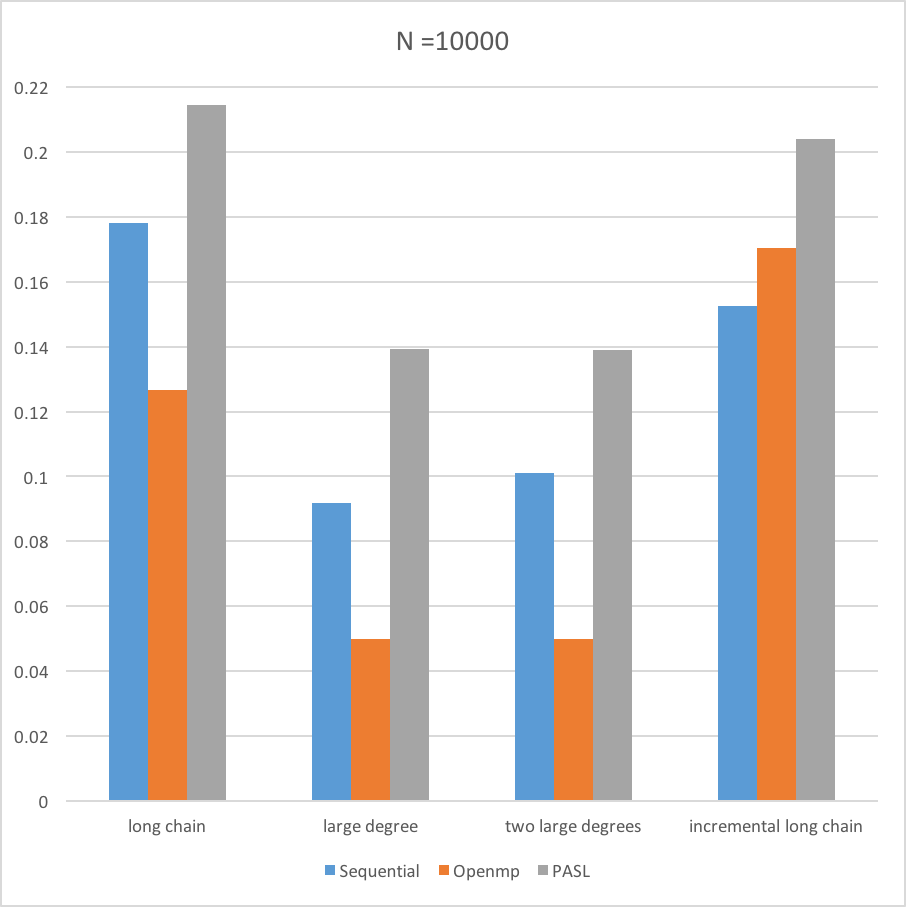
\includegraphics[width=\textwidth]{pic/results-2-a.png}
\end{subfigure}~~\begin{subfigure}[b]{0.45\textwidth}
    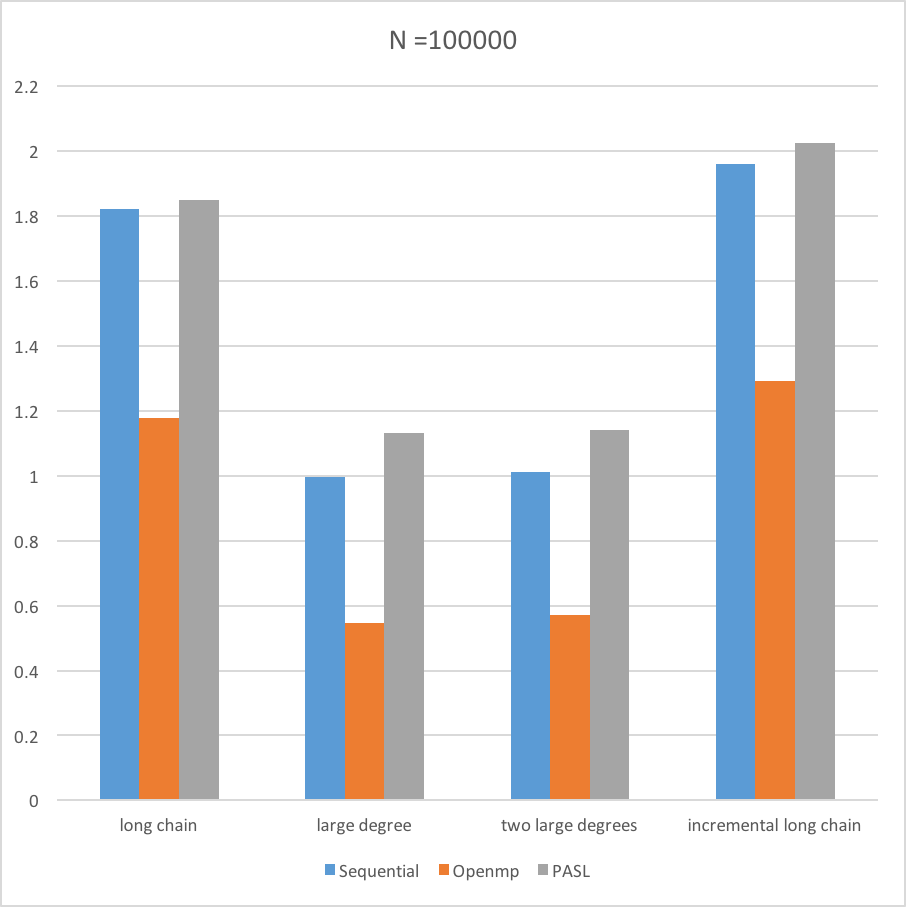
\includegraphics[width=\textwidth]{pic/results-2-b.png}
\end{subfigure}\\
\begin{subfigure}[b]{0.45\textwidth}
    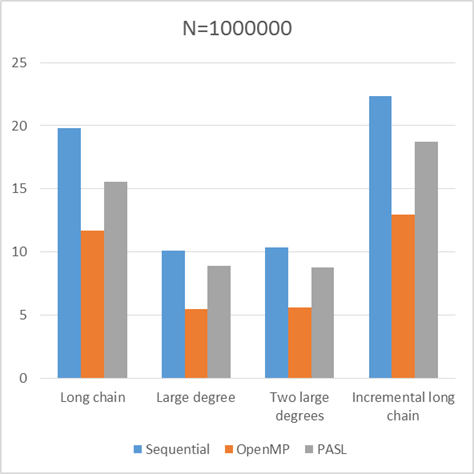
\includegraphics[width=\textwidth]{pic/results-2-c.png}
\end{subfigure}~~\begin{subfigure}[b]{0.45\textwidth}
    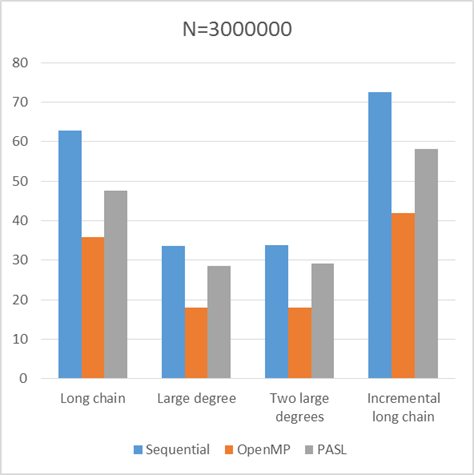
\includegraphics[width=\textwidth]{pic/results-2-d.png}
\end{subfigure}
\caption{Сравнение результатов, два процессора}\label{fig:results-comparison-2}
\end{figure}

\begin{figure}[!ht]
\centering
\begin{subfigure}[b]{0.45\textwidth}
    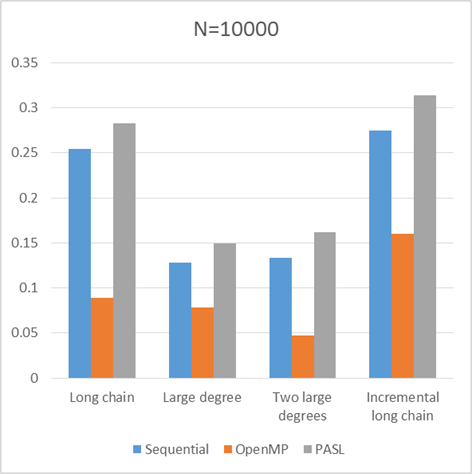
\includegraphics[width=\textwidth]{pic/results-4-a.png}
\end{subfigure}~~\begin{subfigure}[b]{0.45\textwidth}
    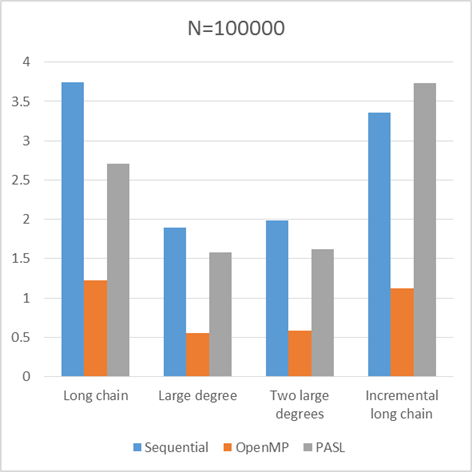
\includegraphics[width=\textwidth]{pic/results-4-b.png}
\end{subfigure}\\
\begin{subfigure}[b]{0.45\textwidth}
    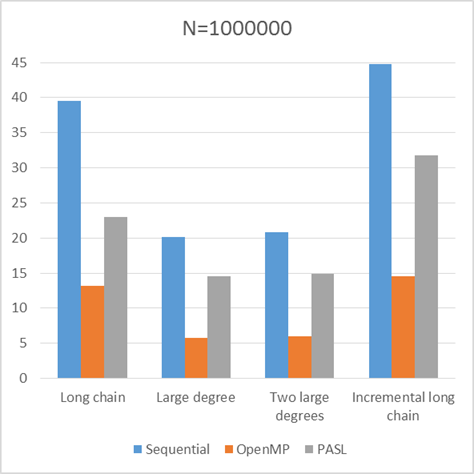
\includegraphics[width=\textwidth]{pic/results-4-c.png}
\end{subfigure}~~\begin{subfigure}[b]{0.45\textwidth}
    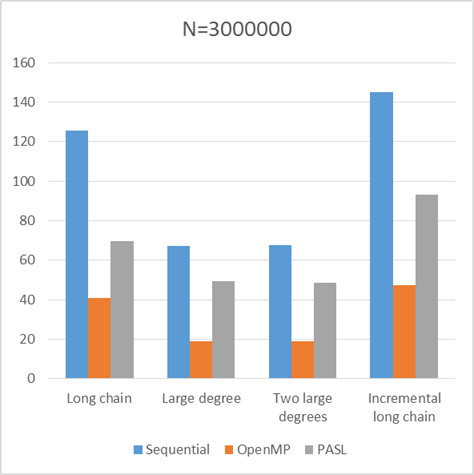
\includegraphics[width=\textwidth]{pic/results-4-d.png}
\end{subfigure}
\caption{Сравнение результатов, четыре процессора}\label{fig:results-comparison-4}
\end{figure}

\revise{
На чертежах, умножить время последовательного вычисления с числом процессоров в качестве справочного материала. Как показывают цифры, в общем смысле, OpenMP лучше, чем PASL в изменяемых процессорах.
}

\chapterconclusion

%% Макрос для заключения. Совместим со старым стилевиком.
\startconclusionpage

\revise{
После тестирования алгоритма, структура данных может поддерживать общий тип данных и данных некоммутативными типа, как и матрица. Реализация структуры данных поддерживает последовательные операции и 
параллельной работы. С улучшением от исходной структуры данных RC-Trees, новый алгоритм работает эффективно. Из оценки, то ясно, что параллельные вычисления с PASL ускоряет все время вычислений и работает 
эффективно. PASL делает большое вычисление данных и вычисление инкрементного изменения более эффективной, чем последовательного вычисления, это означает, что новый алгоритм решает задачу исследования по 
разработке новой структуры данных поддерживает постепенные изменения и быть эффективными. Тем не менее, кажется, что параллельные вычисления с PASL не более эффективен, чем OpenMP в этом эксперименте, в 
результате, параллельная реализация должна быть изменена. Составление использования PASL должна быть оптимизирована. Кроме того, будущая работа будет продолжать оптимизировать алгоритм, чтобы заставить 
его работать более эффективно и стремится работать более эффективно в PASL, чем в OpenMP.
}

%% Обратите внимание на heading. Без него тоже работает, но название будет другим.
\printmainbibliography

\end{document}
